\chapter{}
%\label{chp:appendix}

\section{Further experiment results}

\begin{figure}[!htb]
	\centering
	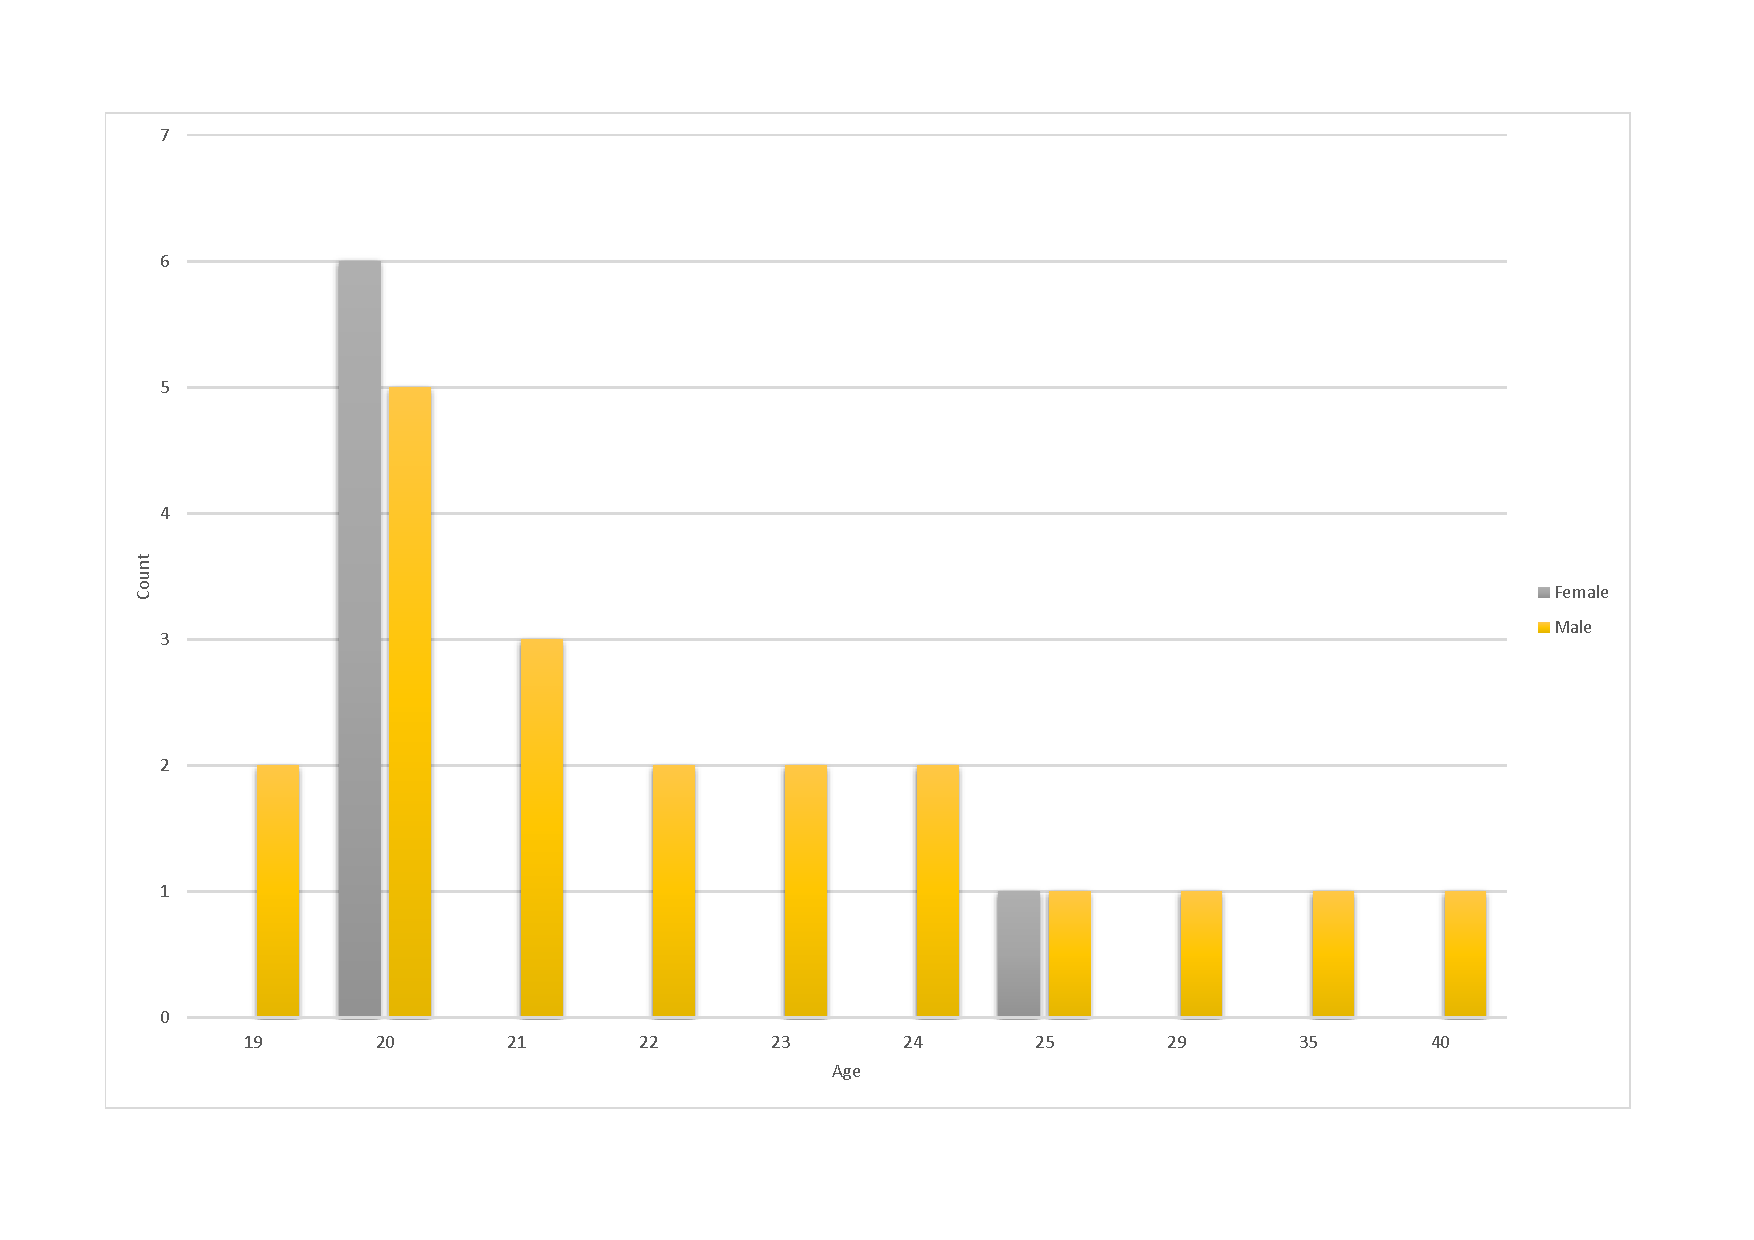
\includegraphics[height=7cm]{charts/genderAge.pdf}
	\caption[Age and gender of experiments particpants]{Count Participants' gender and age }
	\label{fig:chart-genderage}
\end{figure}

\begin{figure}[!htb]
	\centering
	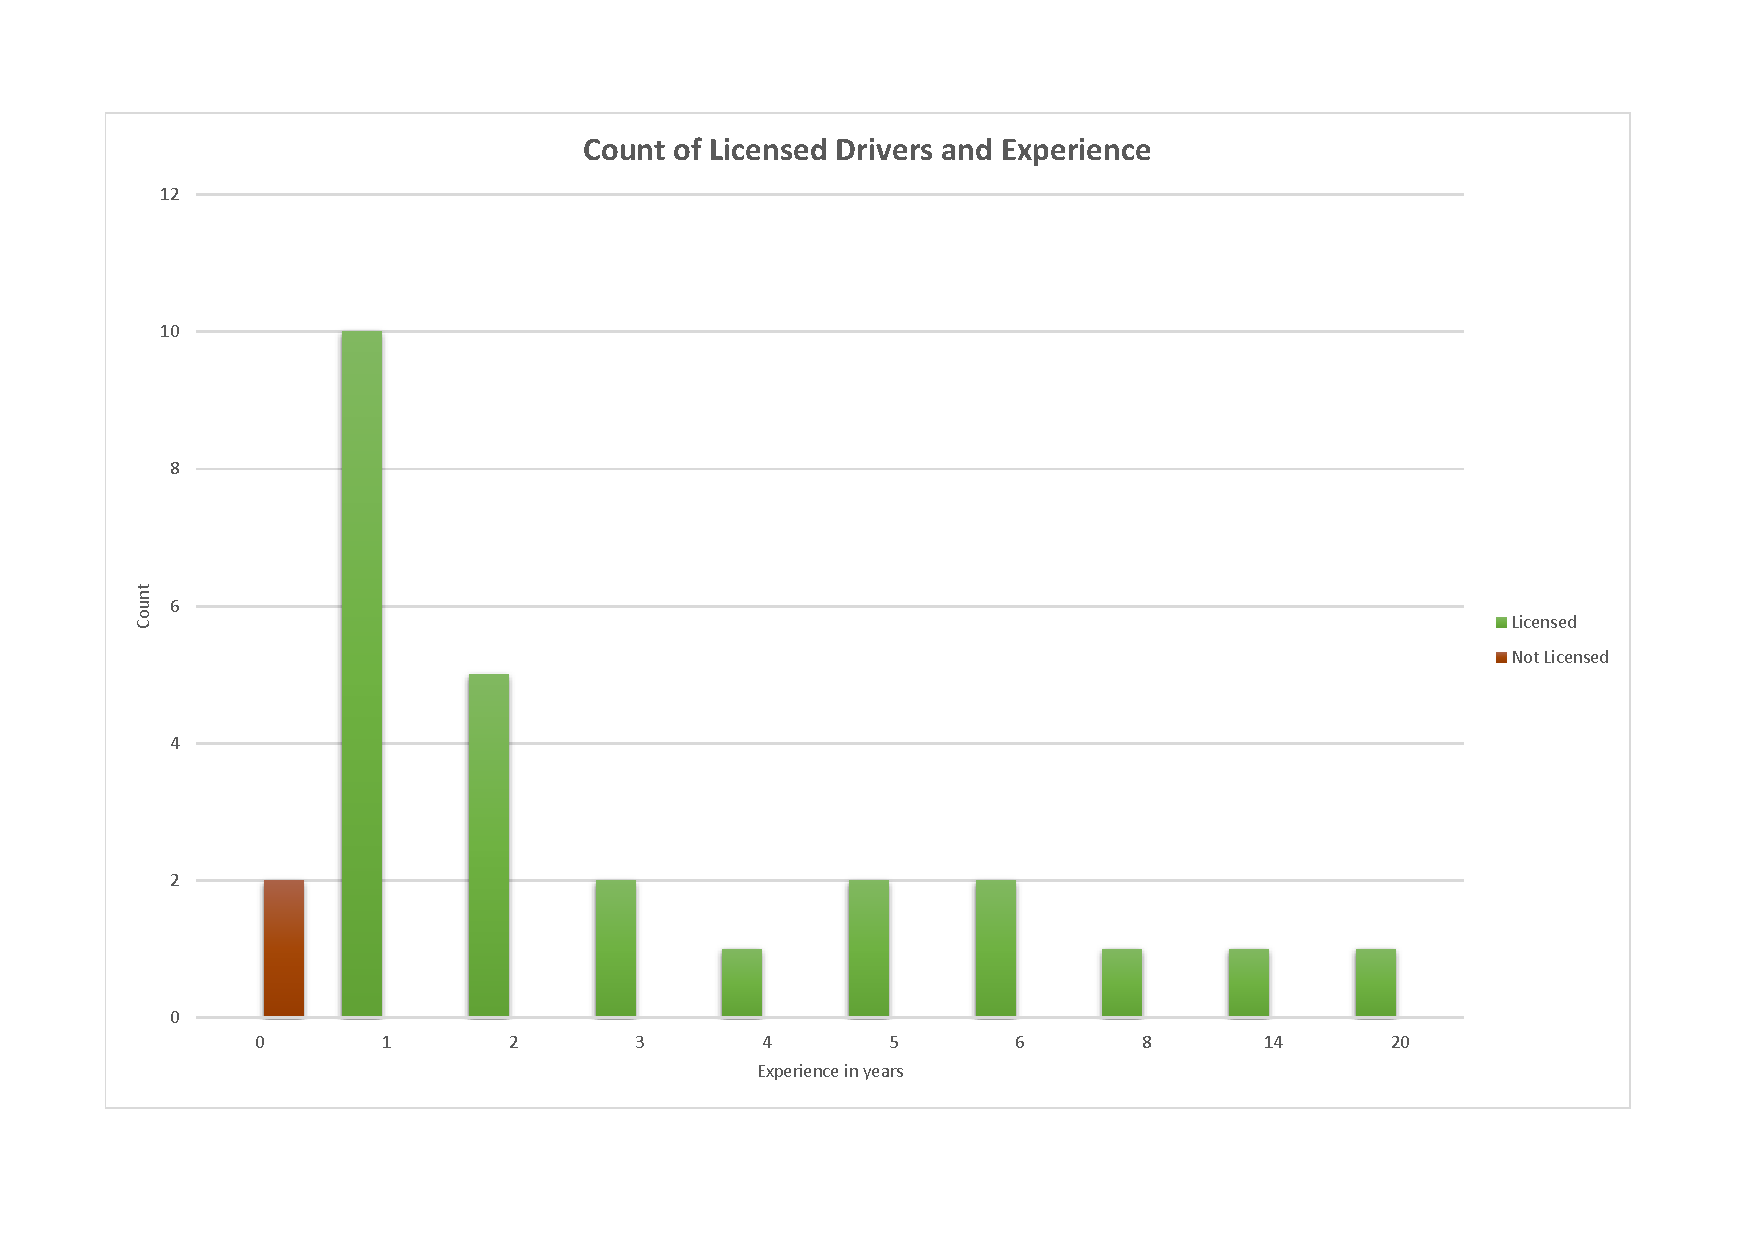
\includegraphics[height=7cm]{charts/licenseddriversexperience.pdf}
	\caption[Particpants Licensed drivers and driving experience]{Licensed drivers and experience}
	\label{fig:chart-licenseddriversexperience}
\end{figure}

\begin{figure}
	\centering
	\begin{minipage}{0.45\textwidth}
		\centering
		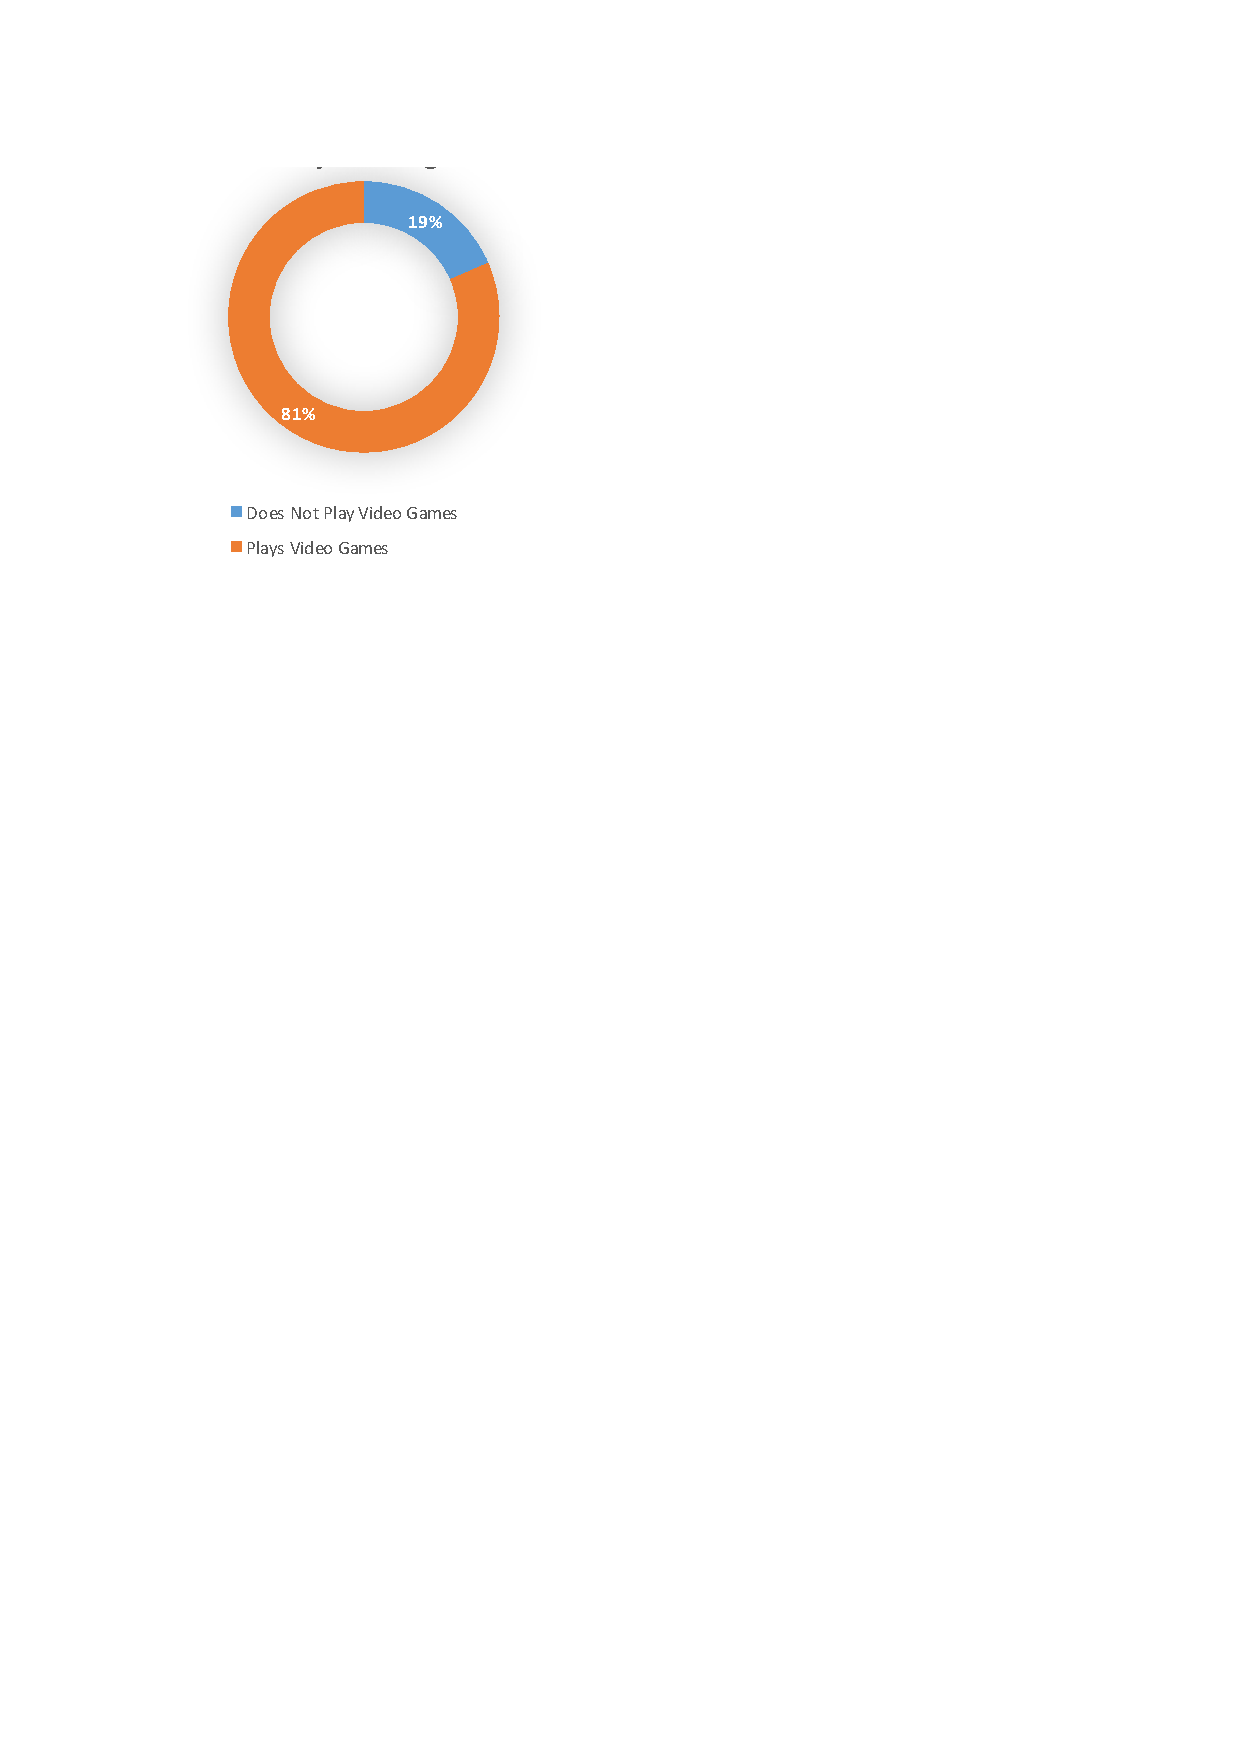
\includegraphics[width=\textwidth]{charts/playVideoGames.pdf}
		\caption[Do particpants play video games?]{Do particpants play video games?}
		\label{fig:chart-playVideoGames}
	\end{minipage}\hfill
	\begin{minipage}{0.45\textwidth}
		\centering
		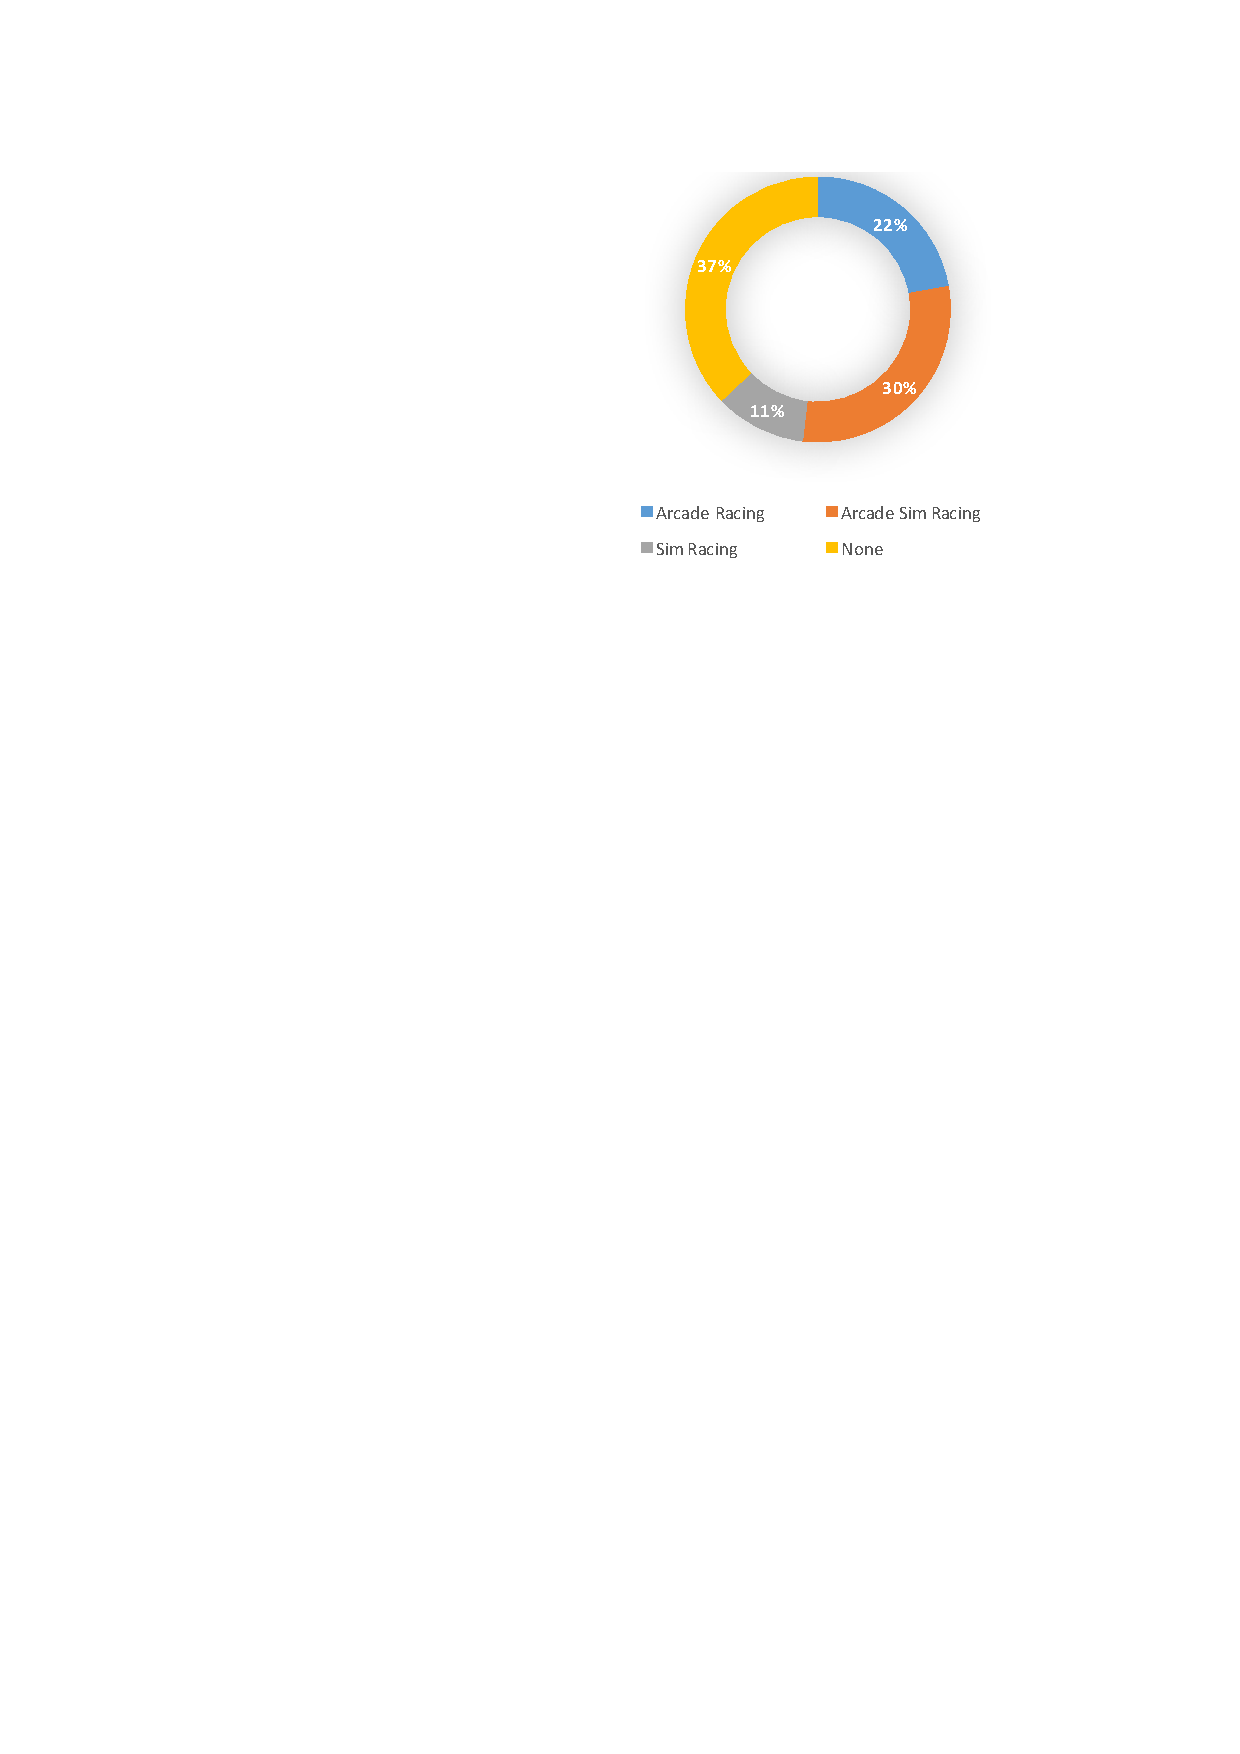
\includegraphics[width=\textwidth]{charts/gamesGenrePlayed.pdf}
		\caption[Racing games genre played by particpants]{Racing games genre played by particpants}
		\label{fig:chart-gamesGenrePlayed}
	\end{minipage}
\end{figure}

\begin{figure}
	\centering
	\begin{minipage}{0.45\textwidth}
		\centering
		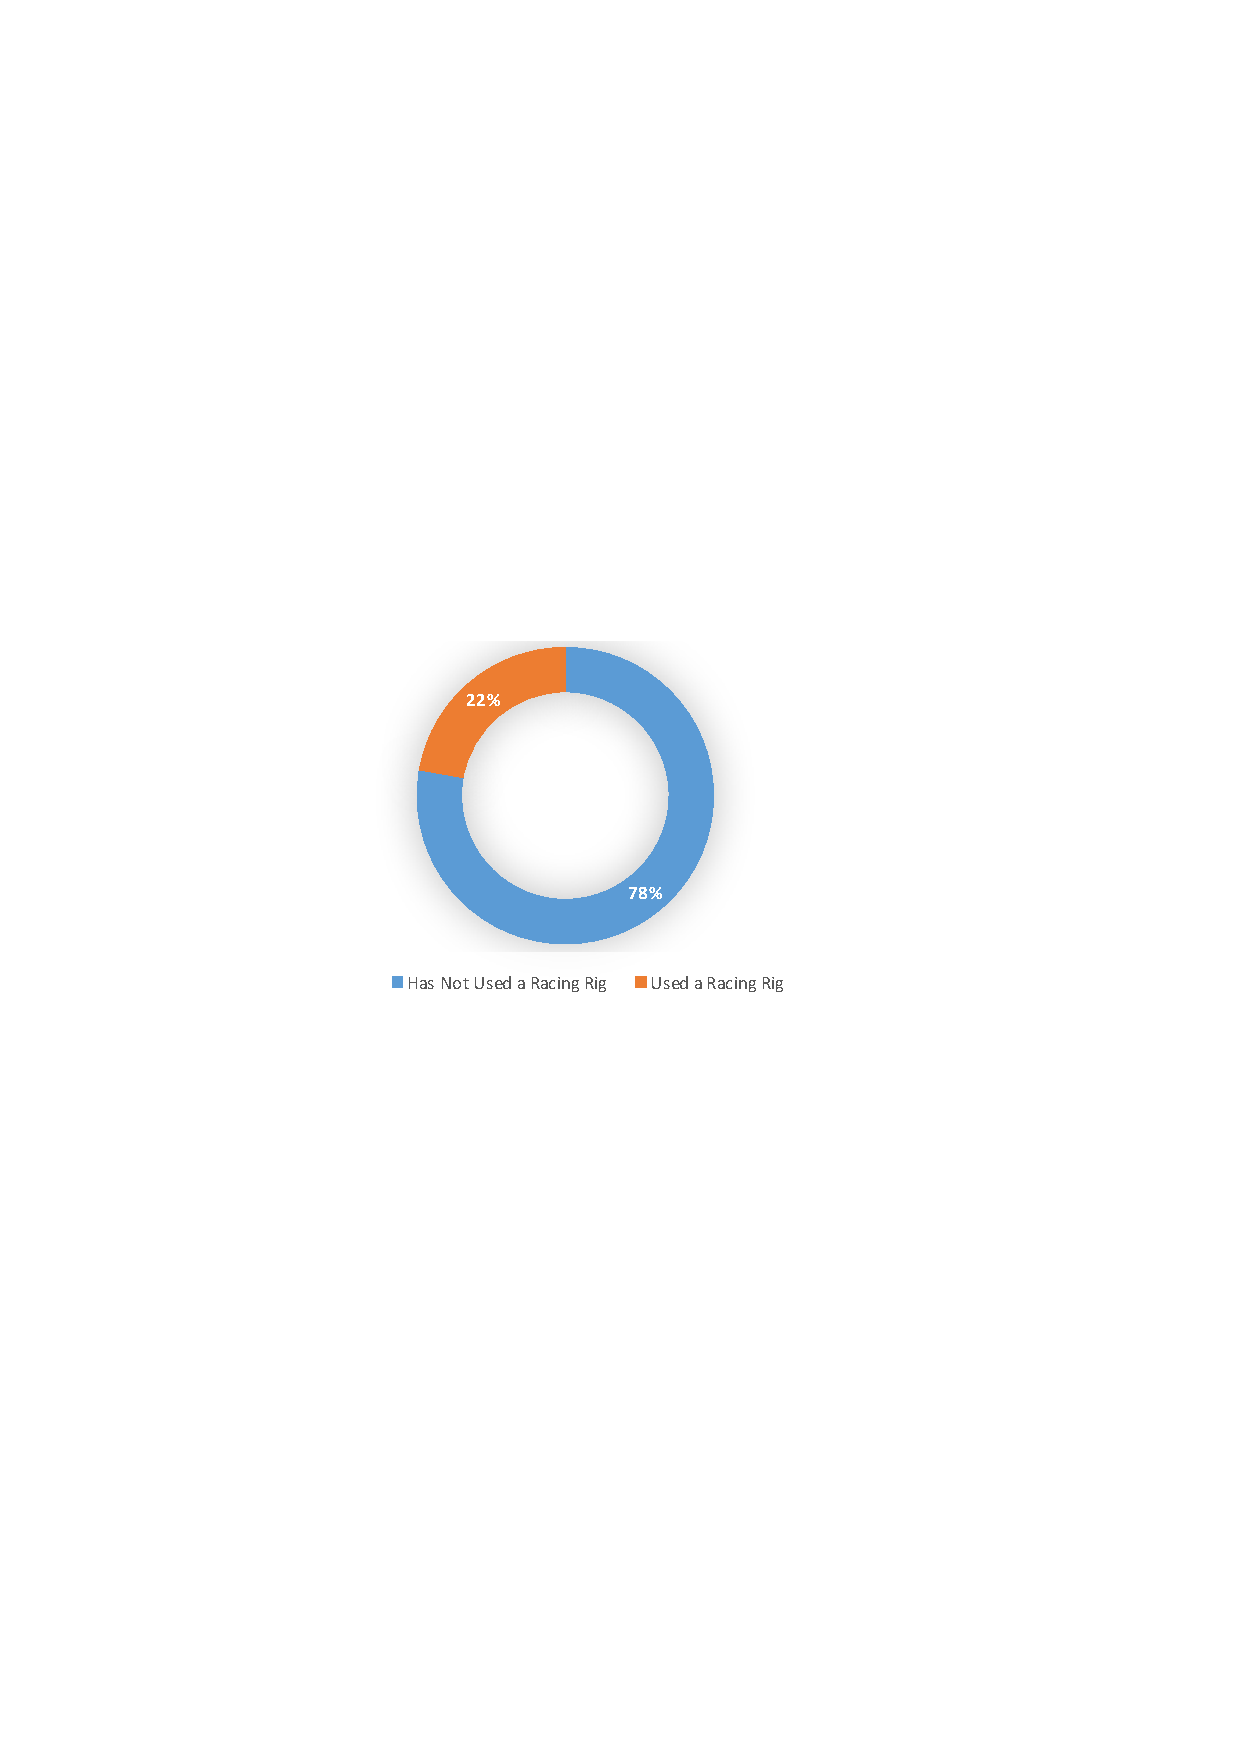
\includegraphics[width=\textwidth]{charts/usedARacingRig.pdf}
		\caption[Have particpants used a race rig?]{Have particpants used a race rig before the experiments?}
		\label{fig:chart-usedARacingRig}
	\end{minipage}\hfill
	\begin{minipage}{0.45\textwidth}
		\centering
		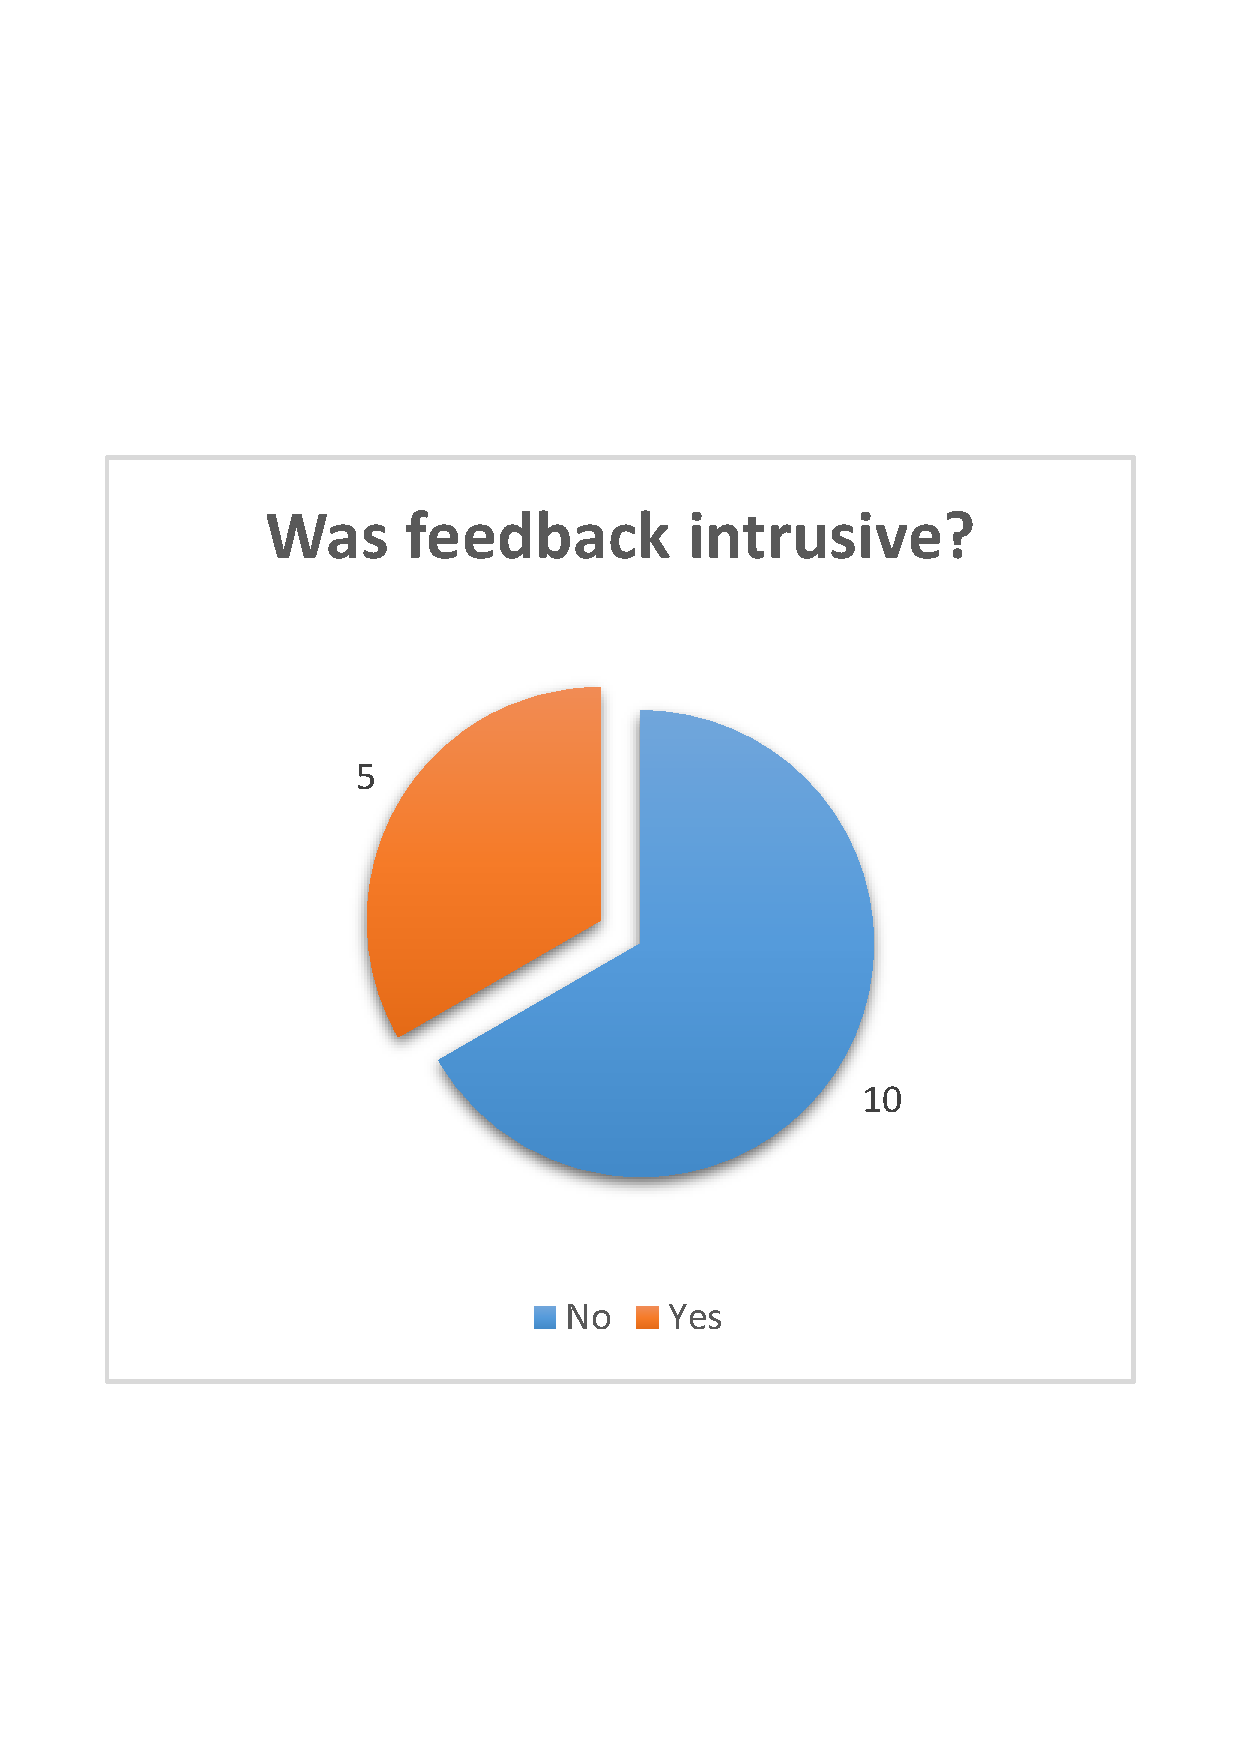
\includegraphics[width=\textwidth]{charts/intrusivefeedback.pdf}
		\caption{Was the feedback intrusive?}
		\label{fig:chart-intrusivefeedback}
	\end{minipage}
\end{figure}

\begin{figure}[!htb]
	\centering
	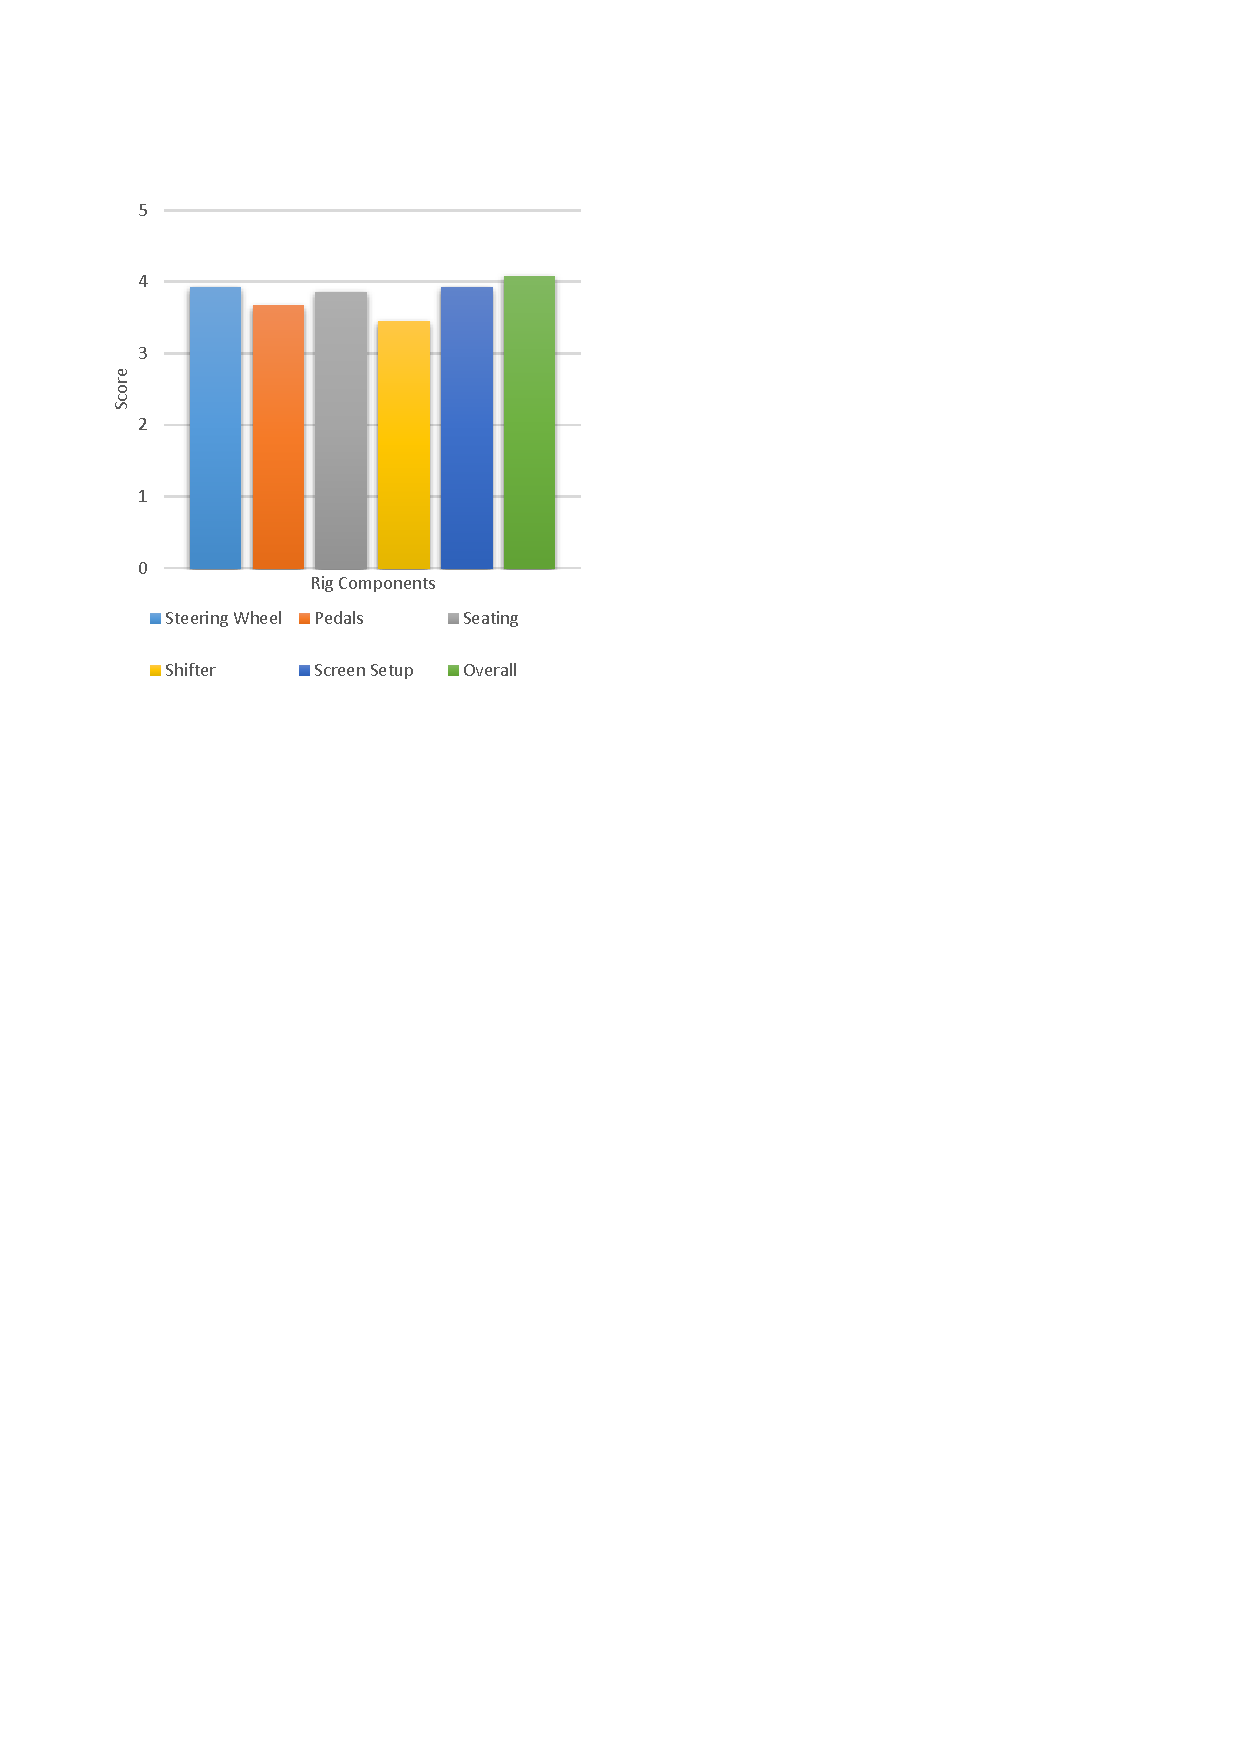
\includegraphics[width=\textwidth]{charts/rigRealisim.pdf}
	\caption[Participants rig realisim score]{How real do these compnets feel?}
	\label{fig:chart-realistic}
\end{figure}

\subsection{Histograms}

This section shows the histograms which have been generated from the dataset which have been used in Chapter \ref{eval}

\begin{figure}
	\figuretitle{Session 1}
	\centering
	\begin{minipage}{0.45\textwidth}
		\centering
		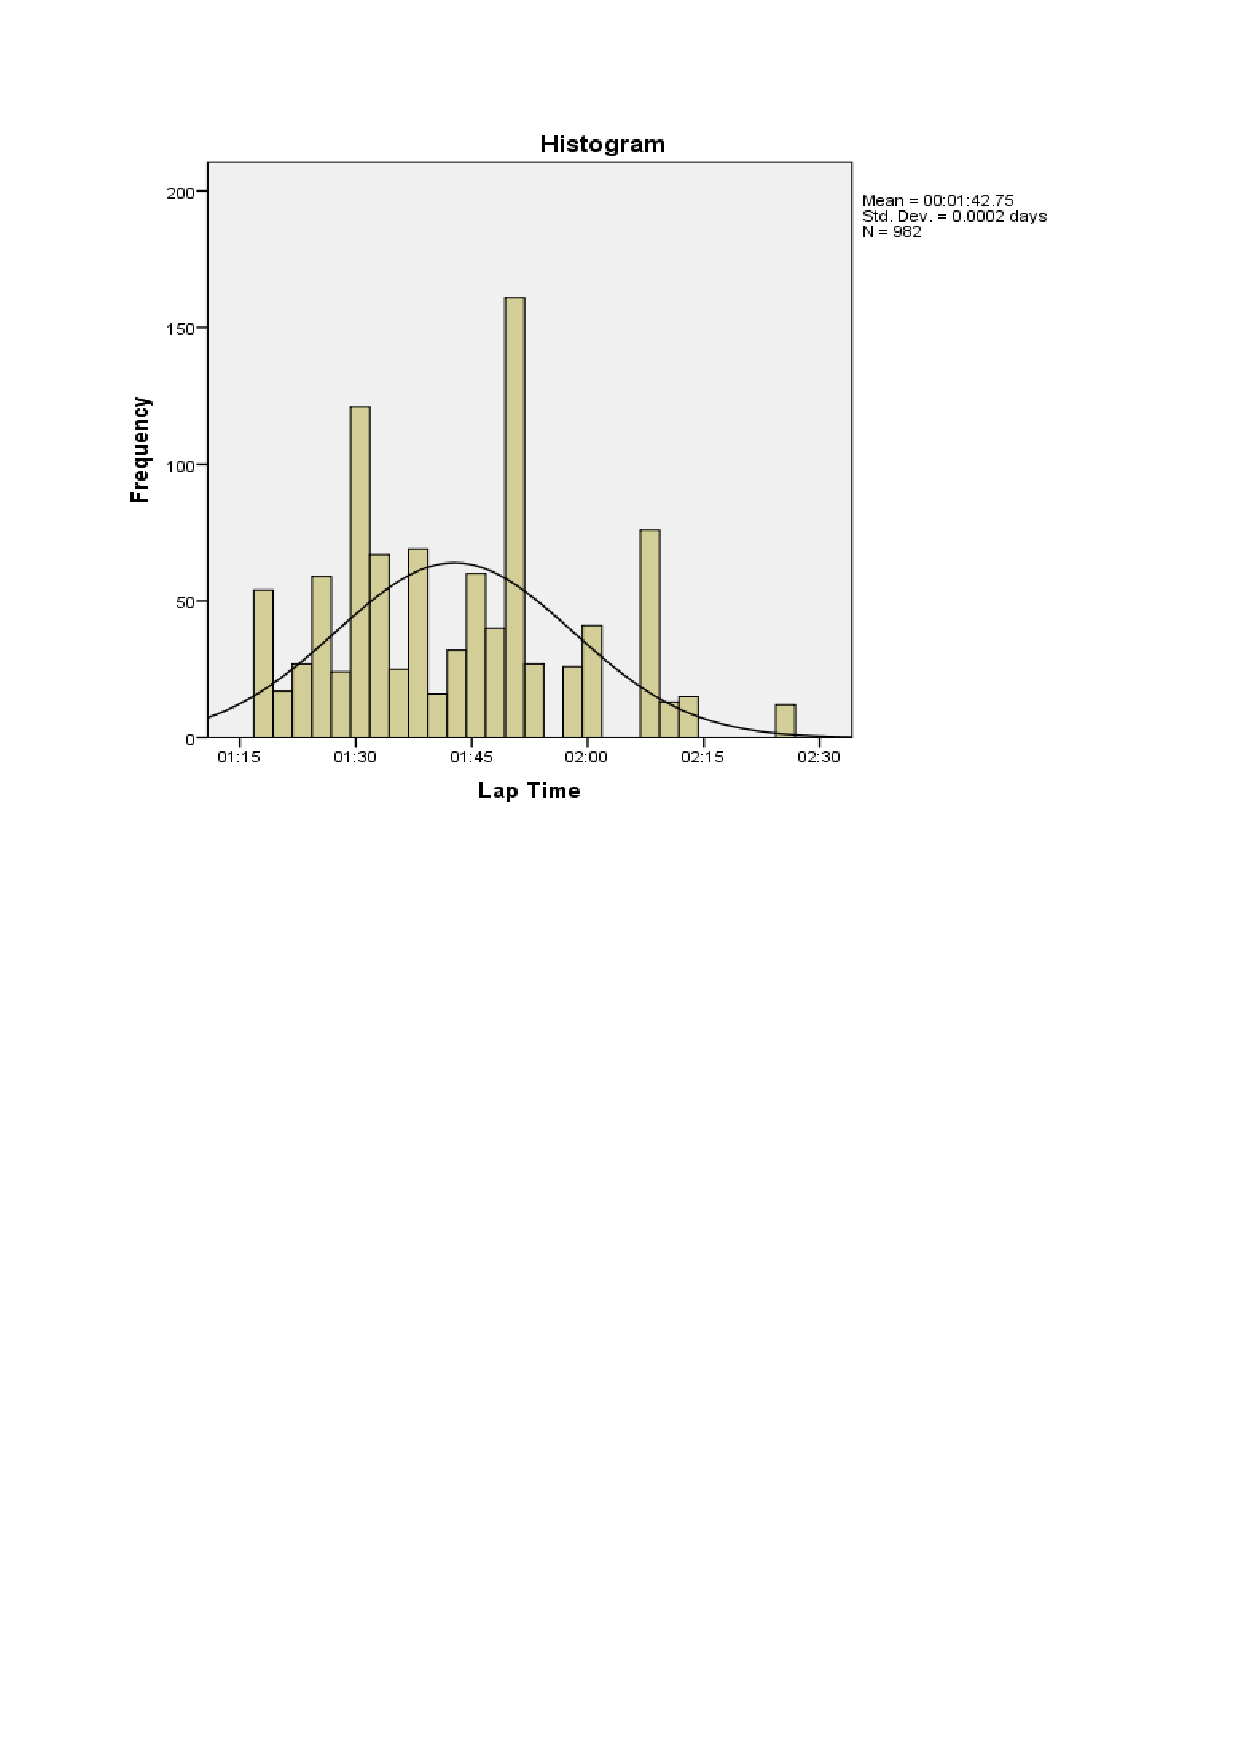
\includegraphics[width=\textwidth]{charts/1-0}
		Control Group
	\end{minipage}\hfill
	\begin{minipage}{0.45\textwidth}
		\centering
		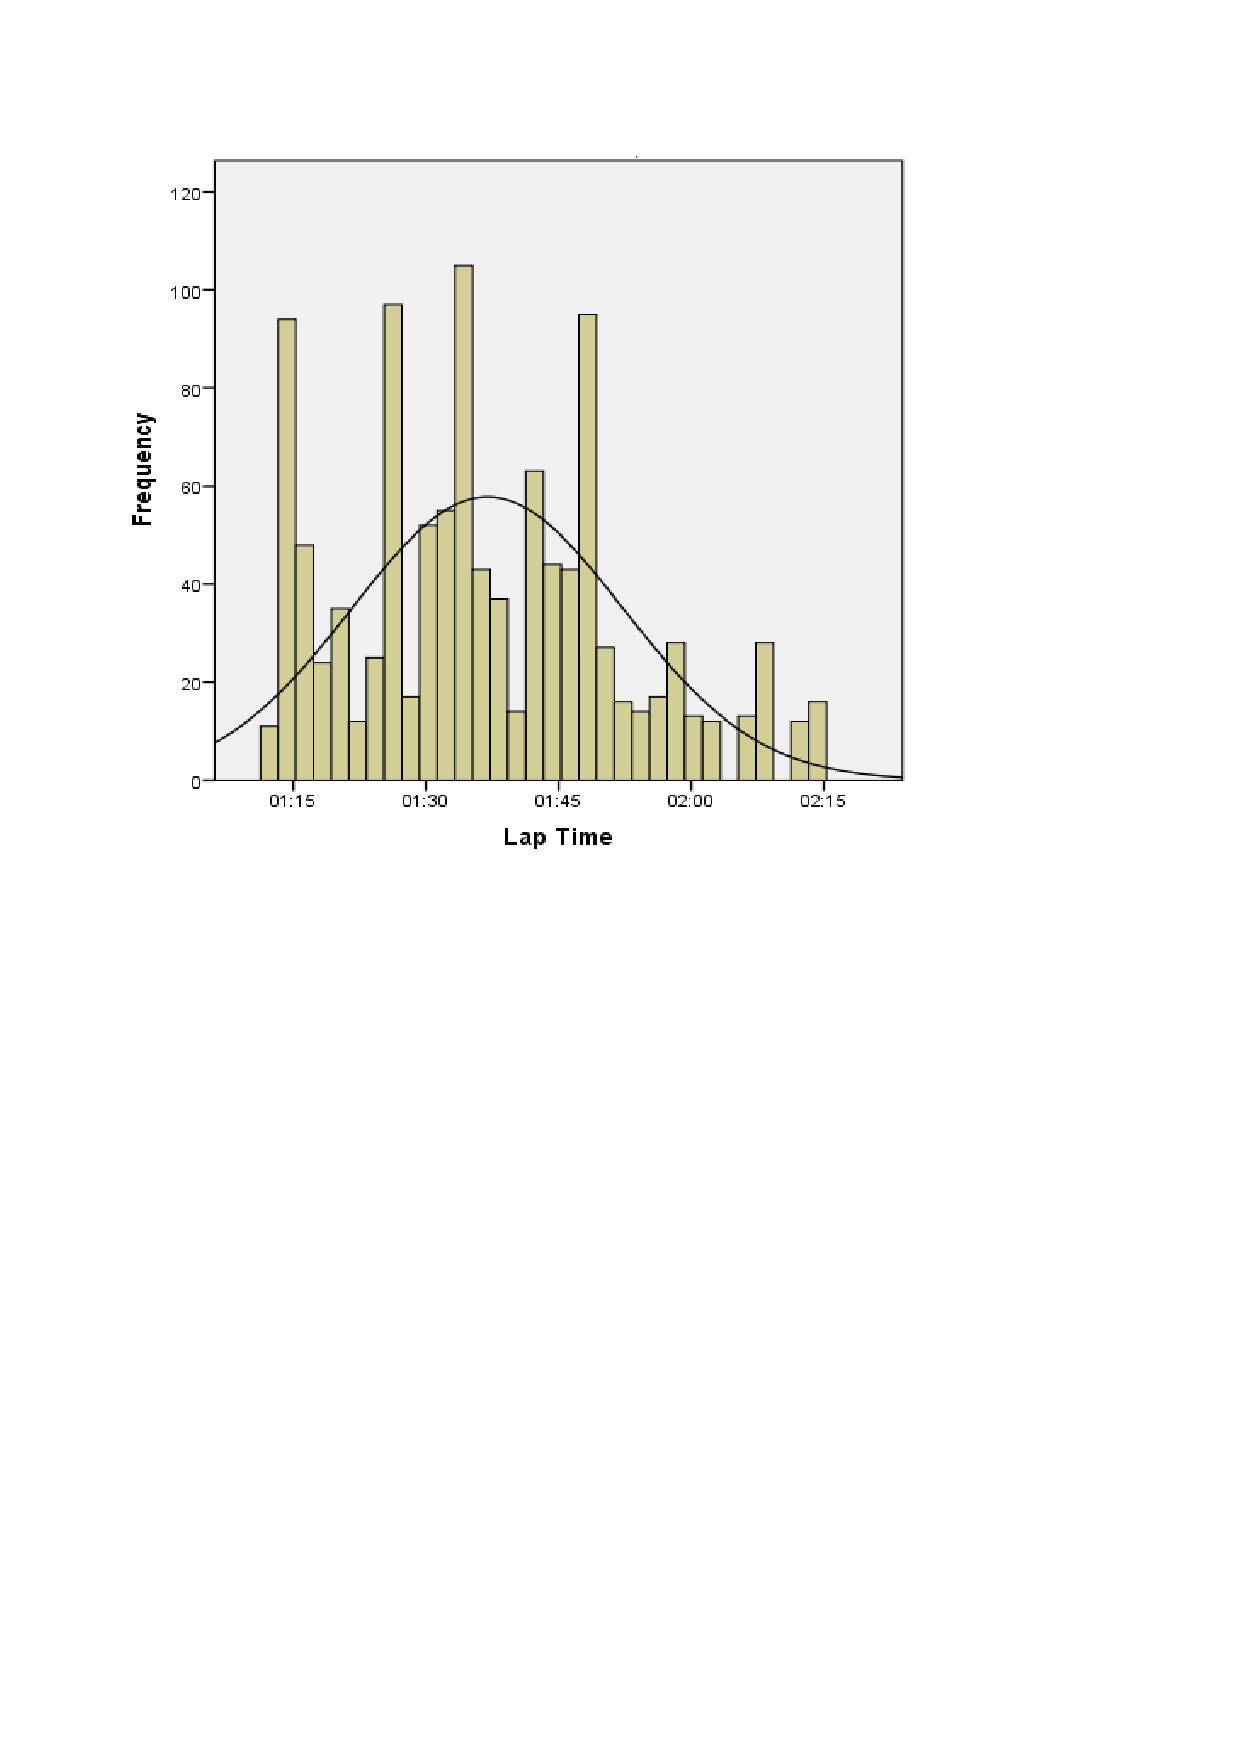
\includegraphics[width=\textwidth]{charts/1-1}
		Feedback Group
	\end{minipage}
	\caption{Histograms generated for the 1st Session}
	\label{fig:hist-1}
\end{figure}

\begin{figure}
	\figuretitle{Session 2}
	\centering
	\begin{minipage}{0.45\textwidth}
		\centering
		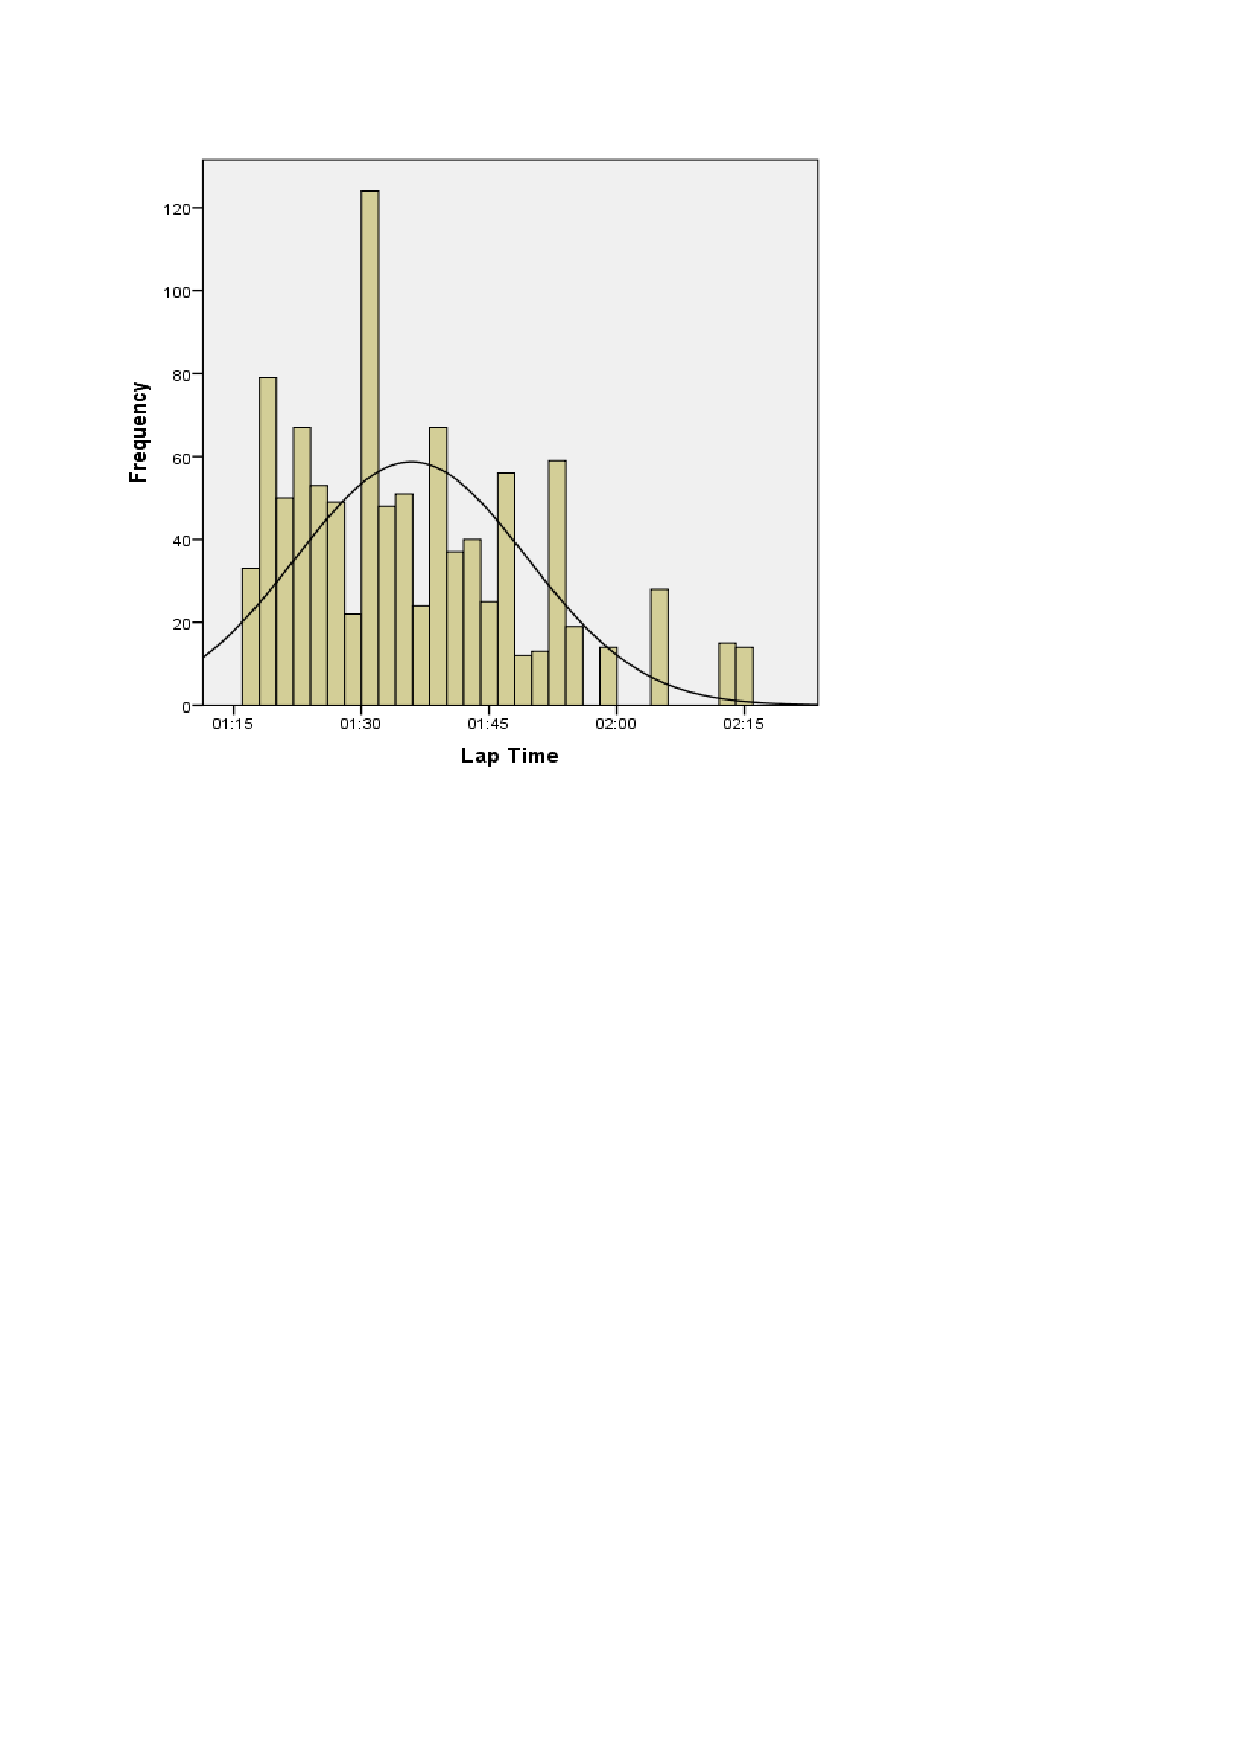
\includegraphics[width=\textwidth]{charts/2-0}
		Control Group
	\end{minipage}\hfill
	\begin{minipage}{0.45\textwidth}
		\centering
		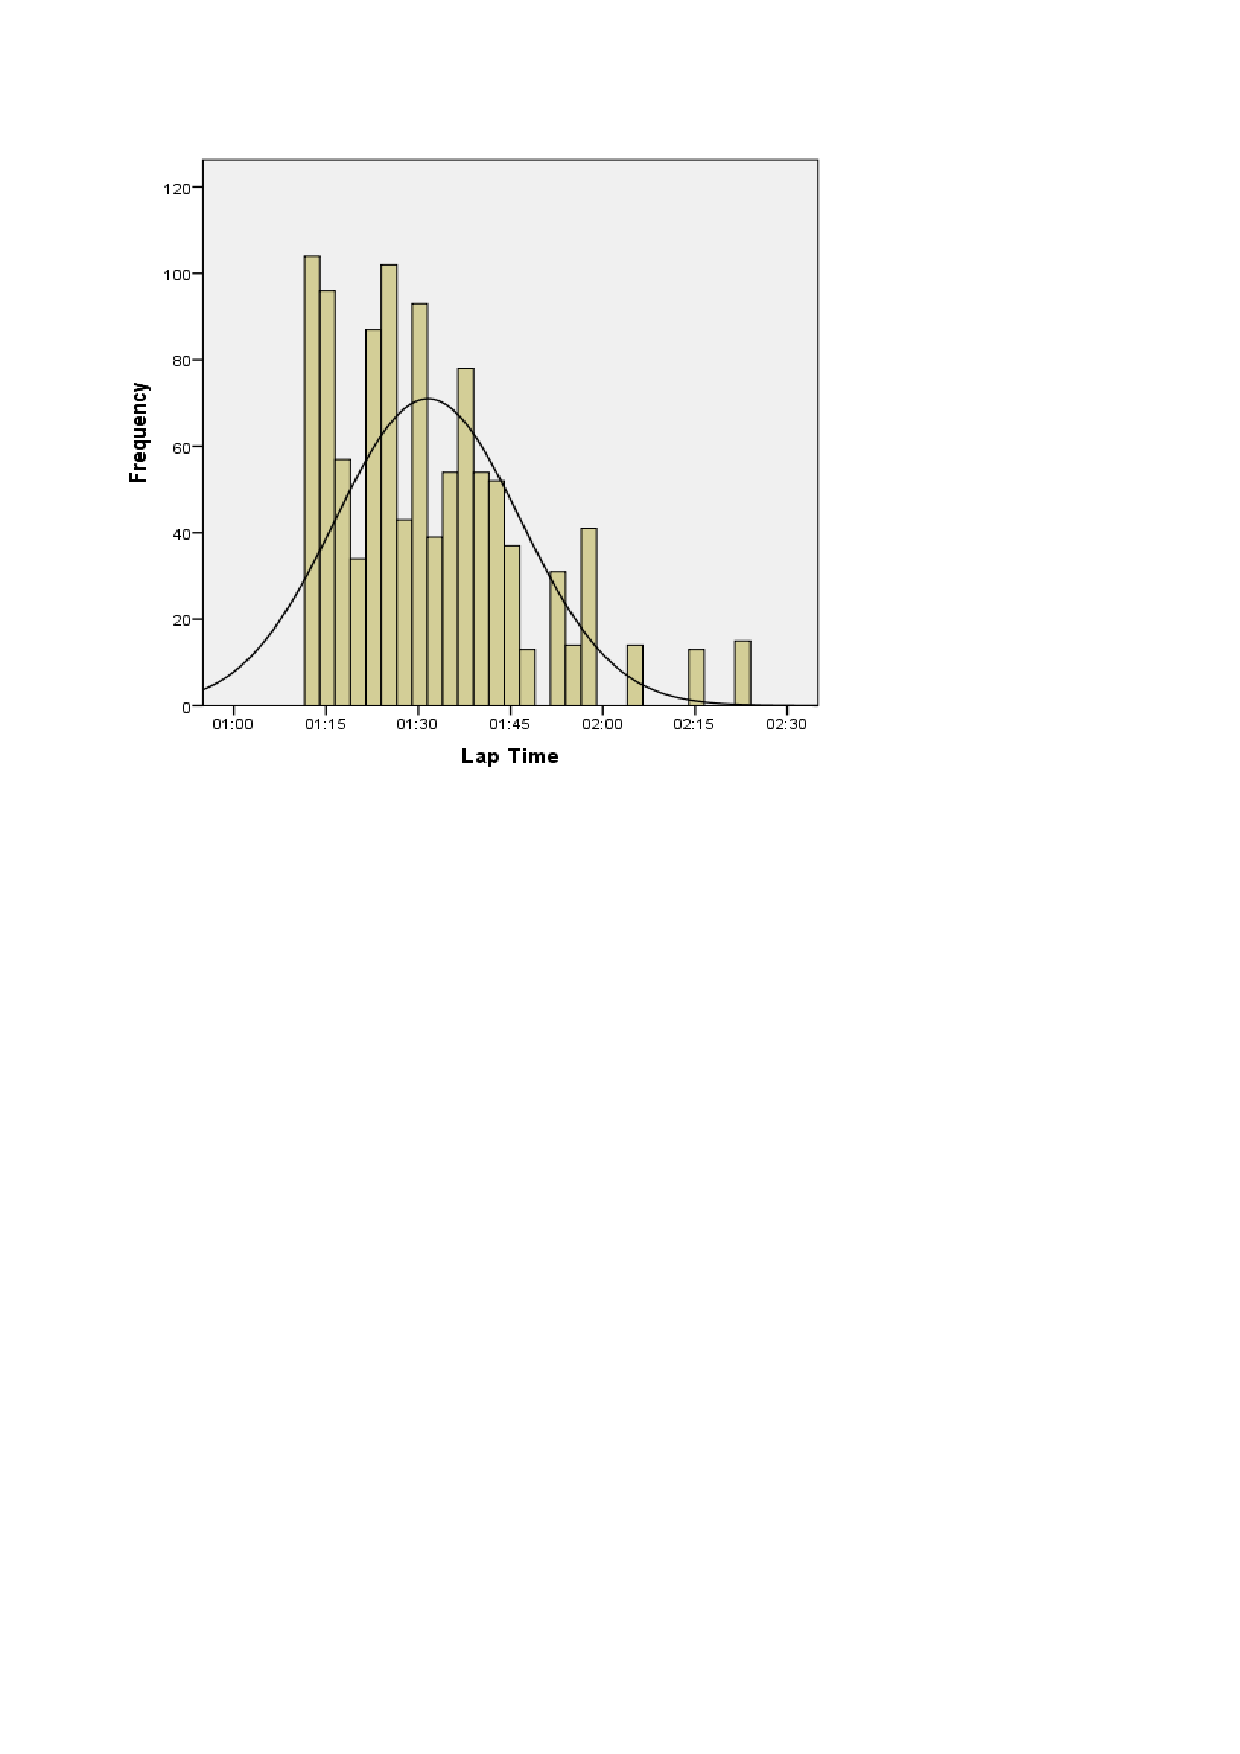
\includegraphics[width=\textwidth]{charts/2-1}
		Feedback Group
	\end{minipage}
	\caption{Histograms generated for the 2nd Session}
	\label{fig:hist-2}
\end{figure}

\begin{figure}
	\figuretitle{Session 3}
	\centering
	\begin{minipage}{0.45\textwidth}
		\centering
		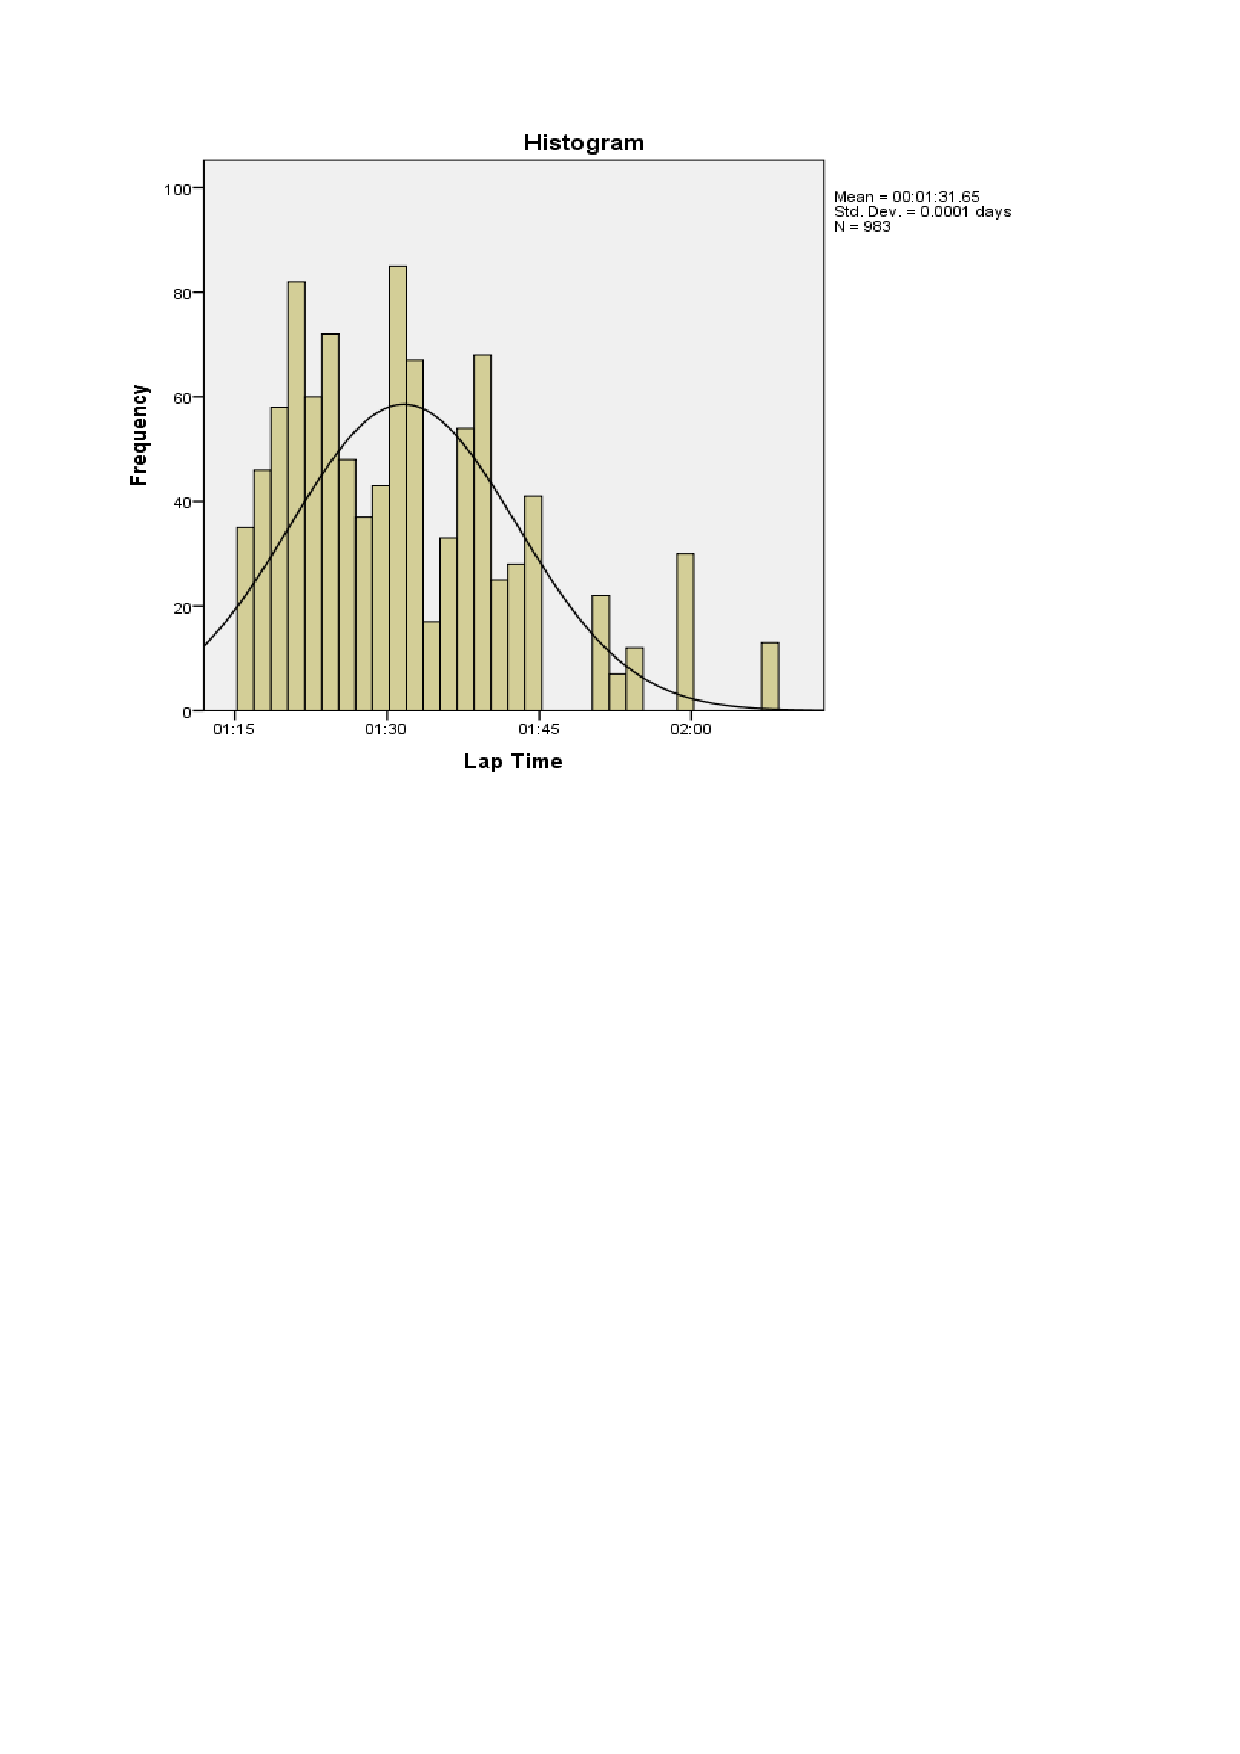
\includegraphics[width=\textwidth]{charts/3-0}
		Control Group
	\end{minipage}\hfill
	\begin{minipage}{0.45\textwidth}
		\centering
		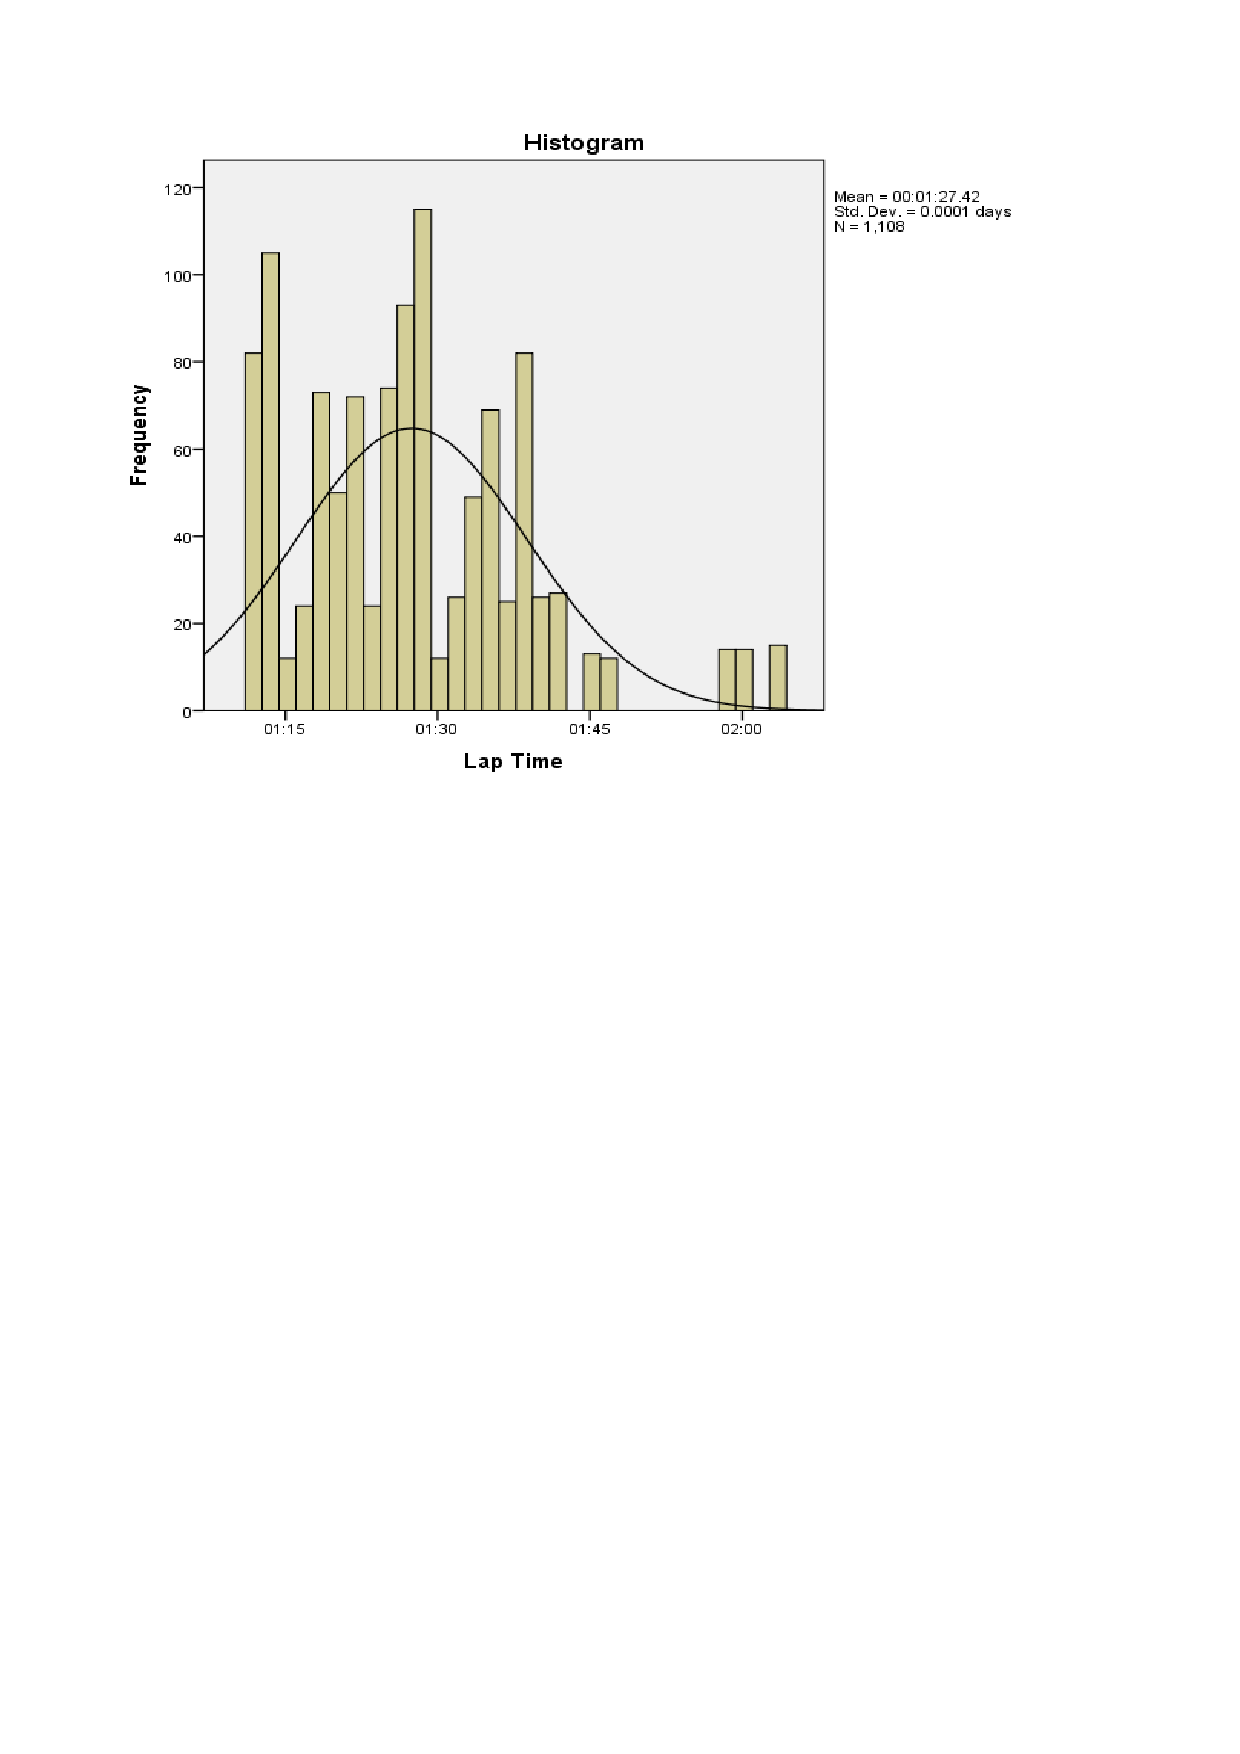
\includegraphics[width=\textwidth]{charts/3-1}
		Feedback Group
	\end{minipage}
	\caption{Histograms generated for the 3rd Session}
	\label{fig:hist-3}
\end{figure}

\begin{figure}
	\figuretitle{Session 4}
	\centering
	\begin{minipage}{0.45\textwidth}
		\centering
		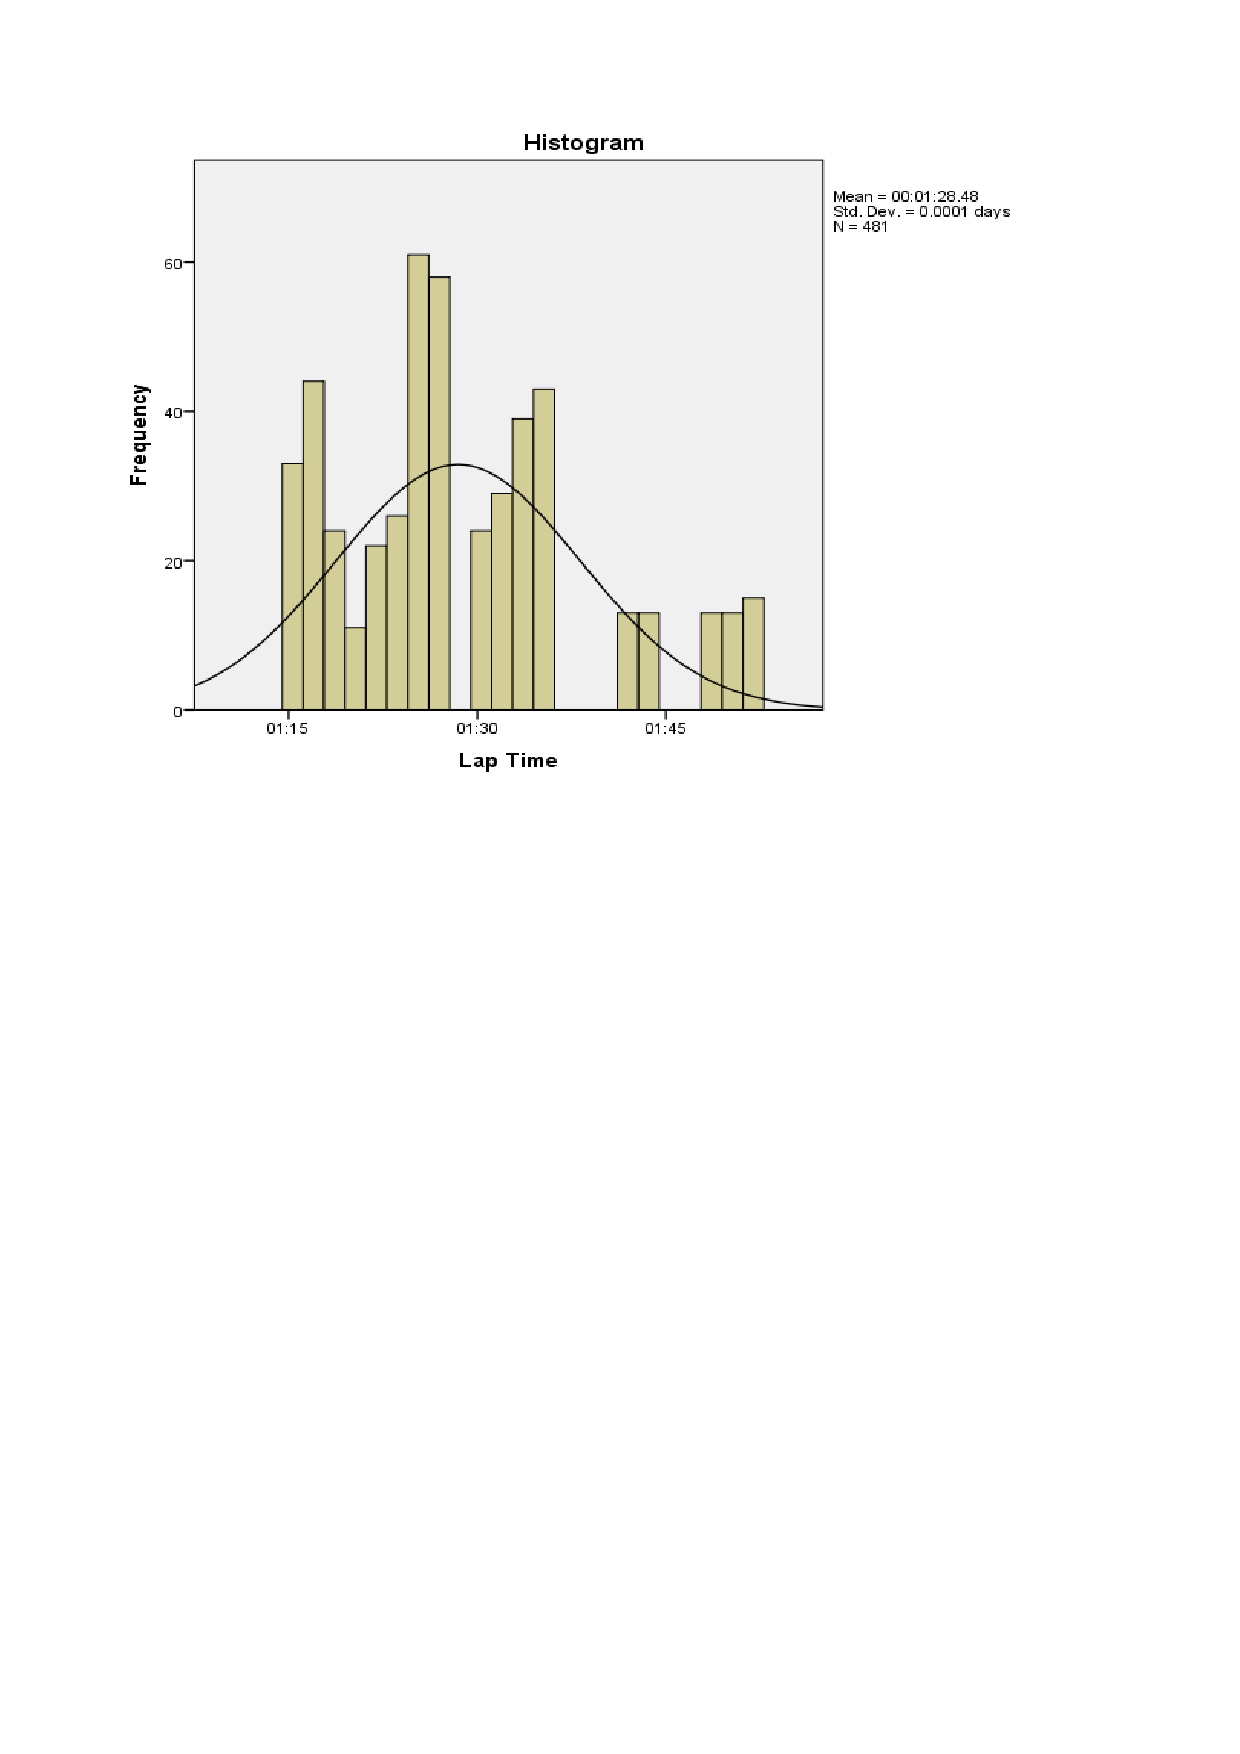
\includegraphics[width=\textwidth]{charts/4-0}
		Control Group
	\end{minipage}\hfill
	\begin{minipage}{0.45\textwidth}
		\centering
		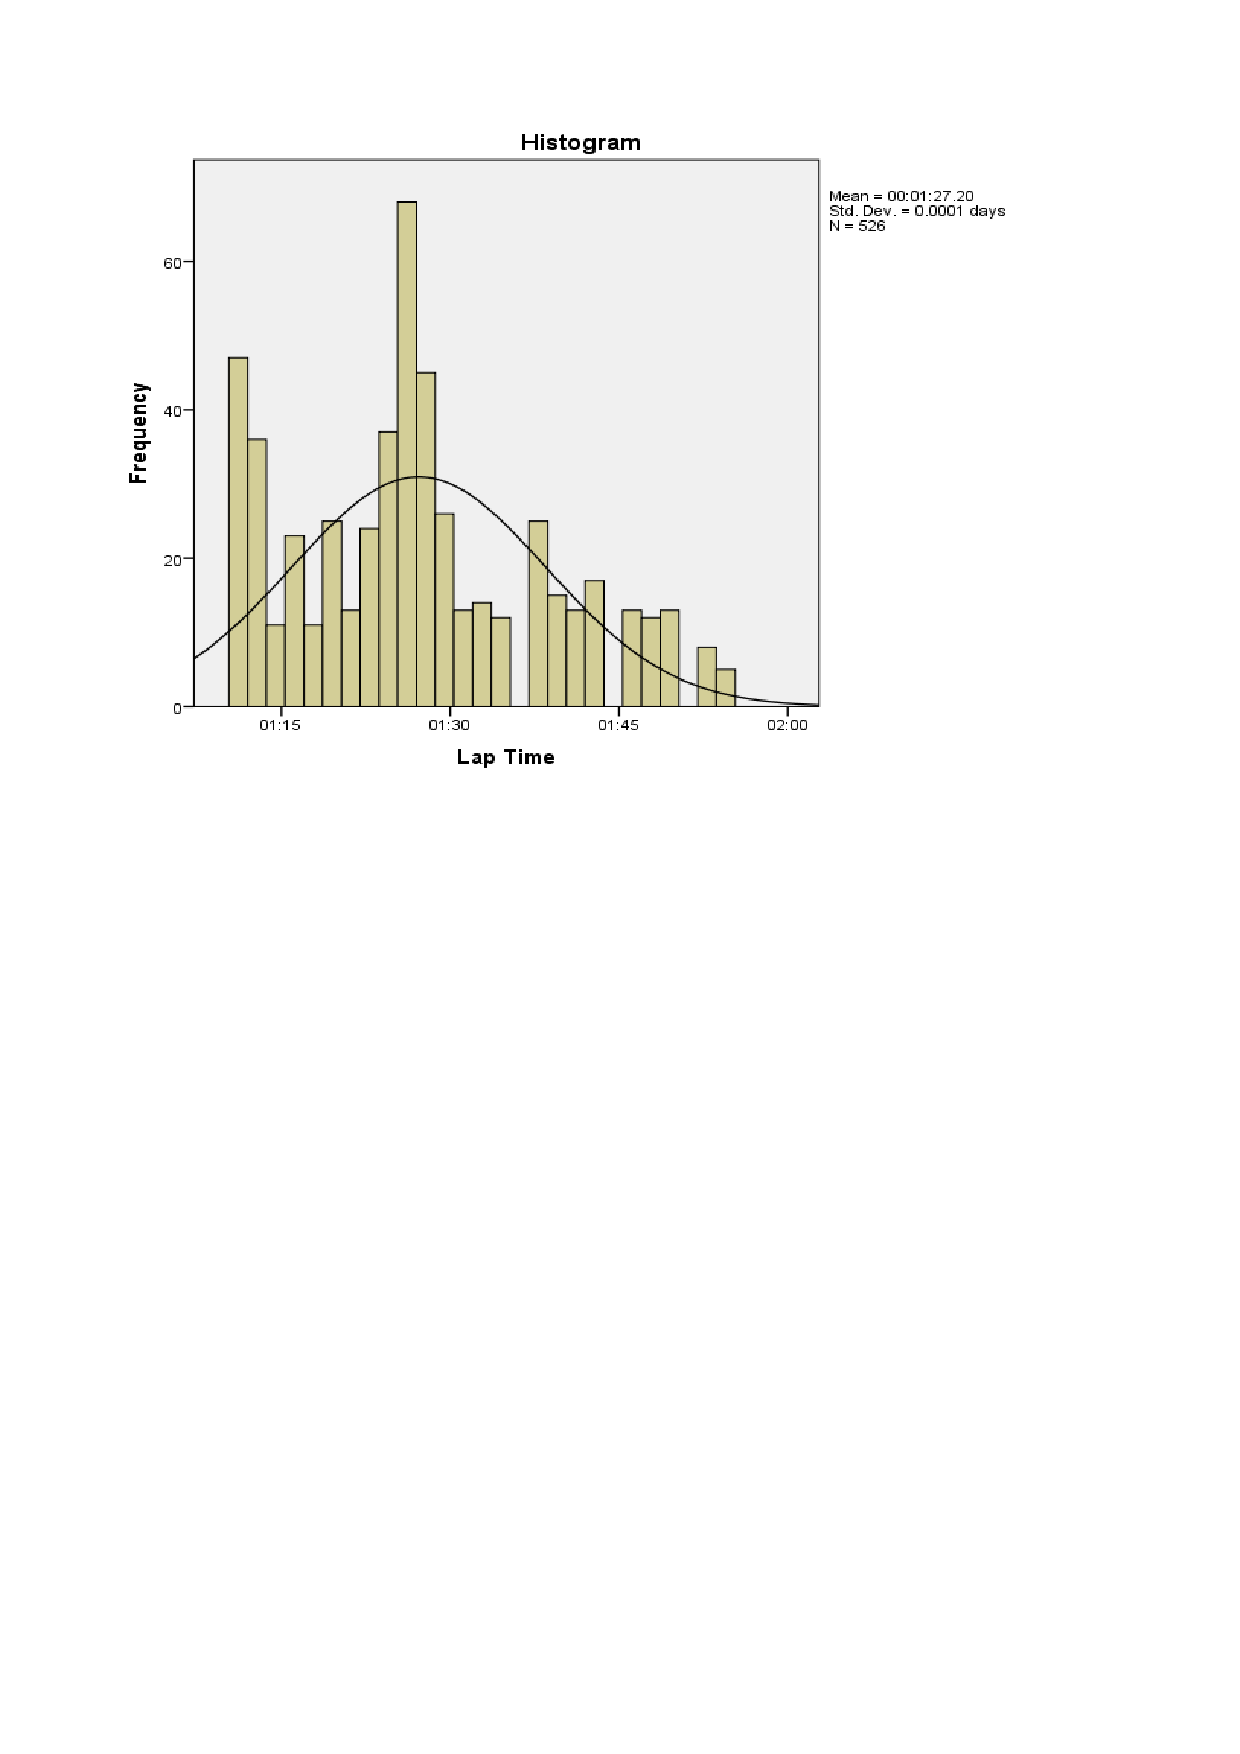
\includegraphics[width=\textwidth]{charts/4-1}
		Feedback Group
	\end{minipage}
	\caption{Histograms generated for the 4th Session}
	\label{fig:hist-4}
\end{figure}

\chapter{}

%
%\section{Questionnaire}
%
%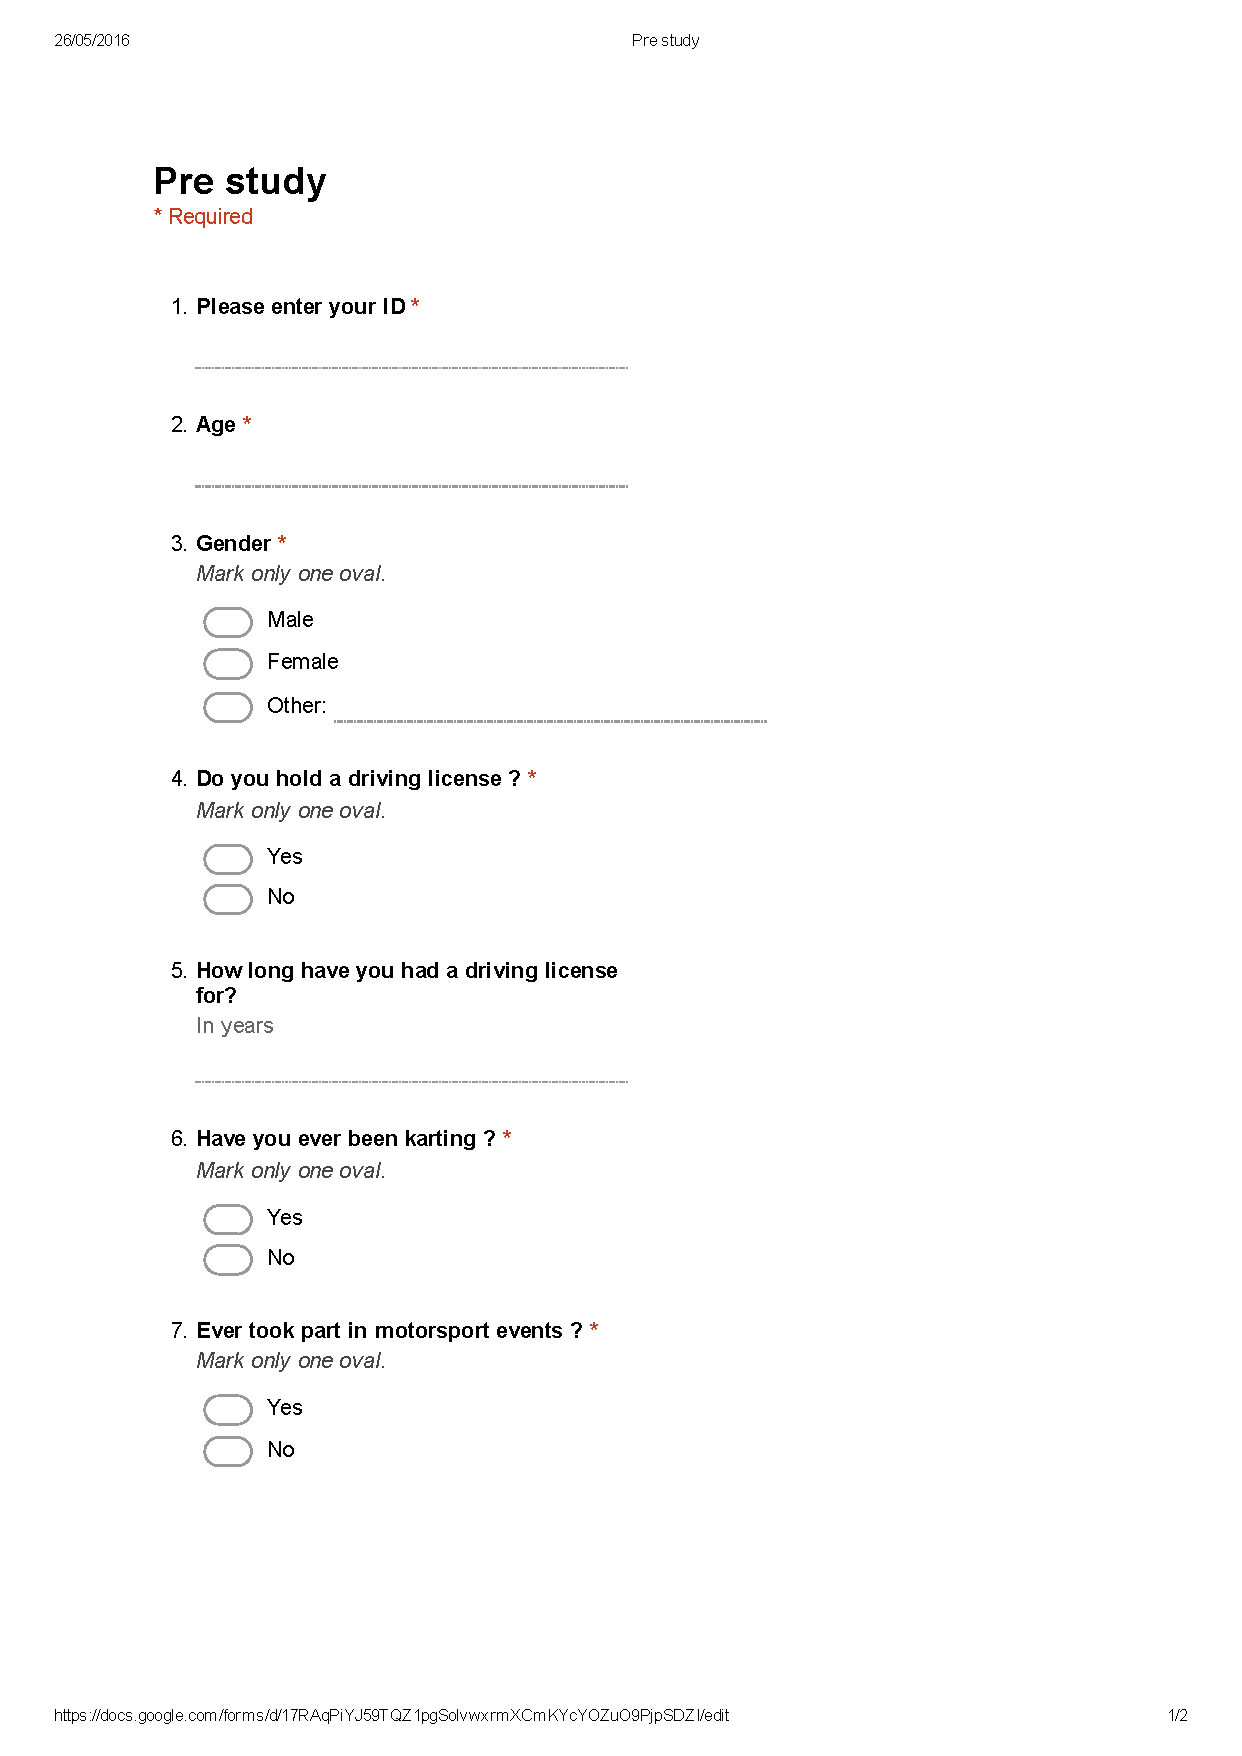
\includepdf[pages=-]{PreStudy.pdf}
%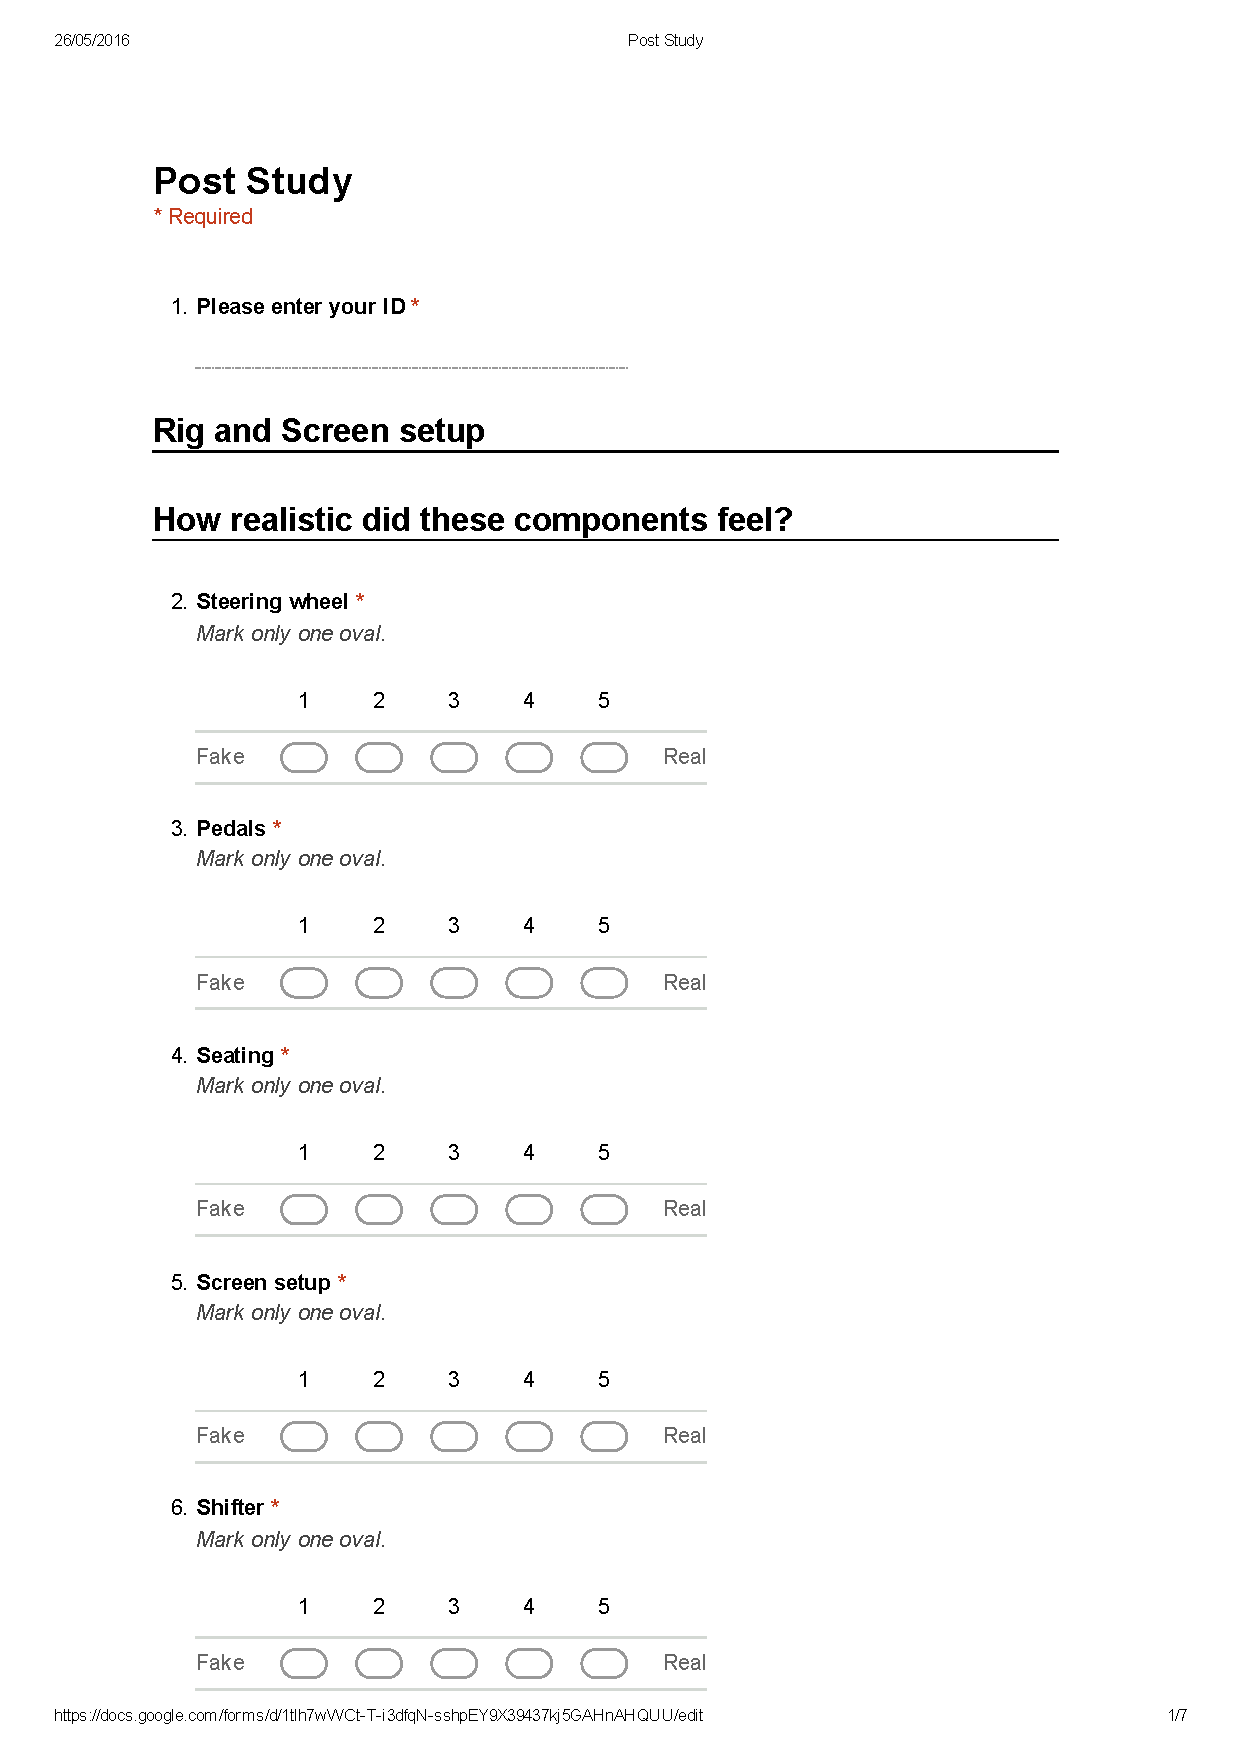
\includepdf[pages=-]{PostStudy.pdf}

\section{Transcript of the feedback audio files}

\begin{description}
	\item [Braking too hard] "Braking too hard"
	\item [Braking too light] "Braking too light"
	\item [Losing traction to the drive wheels by applying too much power] "Too aggressive, ease off the throttle"
	\item [Braking in corner] "Avoid braking while in a corner"
	\item [Incorrect race line during corner] "Turn in late into a corner, aiming for the inside apex"
	\item [Too aggressive during a corner] "Too aggressive during a corner, try easing off the throttle and using less steering input"
	\item [Too slow during a corner] "Try going faster during corner"
	\item [Changing gear too soon] "Changed gear too soon"
	\item [Changed gear too late] "Changed gear too later"
	\item [Taking too long to transition from one gear to another] "Took to long to change gear"
\end{description}